%% Plantilla pandoc simplificada para mdpi.cls (portada: titulo, autores, simple summary, abstract)
\documentclass[water,article,submit,pdftex,moreauthors]{Definitions/mdpi}

% --- Compatibilidad con el codigo que genera pandoc/knitr ---
\providecommand{\tightlist}{\setlength{\itemsep}{0pt}\setlength{\parskip}{0pt}}
\providecommand{\pandocbounded}[1]{#1}
\makeatletter
\def\maxwidth{\ifdim\Gin@nat@width>\linewidth\linewidth\else\Gin@nat@width\fi}
\def\maxheight{\ifdim\Gin@nat@height>.9\textheight.9\textheight\else\Gin@nat@height\fi}
\makeatother
\setkeys{Gin}{width=\maxwidth,height=\maxheight,keepaspectratio}
\usepackage{color}
\usepackage{fancyvrb}
\newcommand{\VerbBar}{|}
\newcommand{\VERB}{\Verb[commandchars=\\\{\}]}
\DefineVerbatimEnvironment{Highlighting}{Verbatim}{commandchars=\\\{\}}
% Add ',fontsize=\small' for more characters per line
\usepackage{framed}
\definecolor{shadecolor}{RGB}{248,248,248}
\newenvironment{Shaded}{\begin{snugshade}}{\end{snugshade}}
\newcommand{\AlertTok}[1]{\textcolor[rgb]{0.94,0.16,0.16}{#1}}
\newcommand{\AnnotationTok}[1]{\textcolor[rgb]{0.56,0.35,0.01}{\textbf{\textit{#1}}}}
\newcommand{\AttributeTok}[1]{\textcolor[rgb]{0.13,0.29,0.53}{#1}}
\newcommand{\BaseNTok}[1]{\textcolor[rgb]{0.00,0.00,0.81}{#1}}
\newcommand{\BuiltInTok}[1]{#1}
\newcommand{\CharTok}[1]{\textcolor[rgb]{0.31,0.60,0.02}{#1}}
\newcommand{\CommentTok}[1]{\textcolor[rgb]{0.56,0.35,0.01}{\textit{#1}}}
\newcommand{\CommentVarTok}[1]{\textcolor[rgb]{0.56,0.35,0.01}{\textbf{\textit{#1}}}}
\newcommand{\ConstantTok}[1]{\textcolor[rgb]{0.56,0.35,0.01}{#1}}
\newcommand{\ControlFlowTok}[1]{\textcolor[rgb]{0.13,0.29,0.53}{\textbf{#1}}}
\newcommand{\DataTypeTok}[1]{\textcolor[rgb]{0.13,0.29,0.53}{#1}}
\newcommand{\DecValTok}[1]{\textcolor[rgb]{0.00,0.00,0.81}{#1}}
\newcommand{\DocumentationTok}[1]{\textcolor[rgb]{0.56,0.35,0.01}{\textbf{\textit{#1}}}}
\newcommand{\ErrorTok}[1]{\textcolor[rgb]{0.64,0.00,0.00}{\textbf{#1}}}
\newcommand{\ExtensionTok}[1]{#1}
\newcommand{\FloatTok}[1]{\textcolor[rgb]{0.00,0.00,0.81}{#1}}
\newcommand{\FunctionTok}[1]{\textcolor[rgb]{0.13,0.29,0.53}{\textbf{#1}}}
\newcommand{\ImportTok}[1]{#1}
\newcommand{\InformationTok}[1]{\textcolor[rgb]{0.56,0.35,0.01}{\textbf{\textit{#1}}}}
\newcommand{\KeywordTok}[1]{\textcolor[rgb]{0.13,0.29,0.53}{\textbf{#1}}}
\newcommand{\NormalTok}[1]{#1}
\newcommand{\OperatorTok}[1]{\textcolor[rgb]{0.81,0.36,0.00}{\textbf{#1}}}
\newcommand{\OtherTok}[1]{\textcolor[rgb]{0.56,0.35,0.01}{#1}}
\newcommand{\PreprocessorTok}[1]{\textcolor[rgb]{0.56,0.35,0.01}{\textit{#1}}}
\newcommand{\RegionMarkerTok}[1]{#1}
\newcommand{\SpecialCharTok}[1]{\textcolor[rgb]{0.81,0.36,0.00}{\textbf{#1}}}
\newcommand{\SpecialStringTok}[1]{\textcolor[rgb]{0.31,0.60,0.02}{#1}}
\newcommand{\StringTok}[1]{\textcolor[rgb]{0.31,0.60,0.02}{#1}}
\newcommand{\VariableTok}[1]{\textcolor[rgb]{0.00,0.00,0.00}{#1}}
\newcommand{\VerbatimStringTok}[1]{\textcolor[rgb]{0.31,0.60,0.02}{#1}}
\newcommand{\WarningTok}[1]{\textcolor[rgb]{0.56,0.35,0.01}{\textbf{\textit{#1}}}}
\usepackage{fvextra}
\DefineVerbatimEnvironment{Highlighting}{Verbatim}{breaklines,breakanywhere,commandchars=\\\{\}}

%% Titulo y autores
\Title{Evolución del Estado de bienestar de los jóvenes europeos}
\Author{Ignacio Lacruz Mascarós, Nicolás Camacho Albiñana}

%% Simple summary y abstract
\simplesumm{Resumen sencillo para un público no especializado.}
\abstract{Resumen técnico del trabajo.}

%% Referencias
\reftitle{References}
\externalbibliography{yes}

\begin{document}


\section{Importación de los
DataFrames}\label{importaciuxf3n-de-los-dataframes}

\begin{Shaded}
\begin{Highlighting}[]
\FunctionTok{library}\NormalTok{(readr)}
\FunctionTok{library}\NormalTok{(stringr)}
\FunctionTok{library}\NormalTok{(dplyr)}
\FunctionTok{library}\NormalTok{(tidyr)}
\FunctionTok{library}\NormalTok{(magrittr)}
\FunctionTok{library}\NormalTok{(lubridate)}
\FunctionTok{library}\NormalTok{(ggplot2)}
\FunctionTok{library}\NormalTok{(GGally)}
\end{Highlighting}
\end{Shaded}

\begin{Shaded}
\begin{Highlighting}[]
\CommentTok{\# Cargamos el dataframe}
\NormalTok{poblacion }\OtherTok{\textless{}{-}} \FunctionTok{read\_tsv}\NormalTok{(}\StringTok{\textquotesingle{}data/poblacion\_paises.tsv\textquotesingle{}}\NormalTok{)}

\CommentTok{\# Limpiamos los nombres de la variable country para obtener los nombres de los paises}
\FunctionTok{colnames}\NormalTok{(poblacion)[}\DecValTok{1}\NormalTok{] }\OtherTok{\textless{}{-}} \StringTok{\textquotesingle{}country\textquotesingle{}}
\NormalTok{poblacion }\SpecialCharTok{\%\textless{}\textgreater{}\%} \FunctionTok{mutate}\NormalTok{(}\AttributeTok{country =} \FunctionTok{sub}\NormalTok{(}\StringTok{"\^{}.*,"}\NormalTok{, }\StringTok{""}\NormalTok{, country)) }\SpecialCharTok{\%\textgreater{}\%} \FunctionTok{mutate}\NormalTok{(}\FunctionTok{across}\NormalTok{(}\SpecialCharTok{{-}}\DecValTok{1}\NormalTok{, }\SpecialCharTok{\textasciitilde{}} \FunctionTok{as.numeric}\NormalTok{(}\FunctionTok{gsub}\NormalTok{(}\StringTok{\textquotesingle{}[\^{}0{-}9.]\textquotesingle{}}\NormalTok{, }\StringTok{\textquotesingle{}\textquotesingle{}}\NormalTok{, .x))))}

\CommentTok{\# Calculamos la media poblacional de cada pais desde el 2000 hasta hoy}
\NormalTok{poblacion }\SpecialCharTok{\%\textless{}\textgreater{}\%} \FunctionTok{transmute}\NormalTok{(country, }\AttributeTok{population =} \FunctionTok{rowMeans}\NormalTok{(}\FunctionTok{select}\NormalTok{(., }\SpecialCharTok{{-}}\NormalTok{country), }\AttributeTok{na.rm =} \ConstantTok{TRUE}\NormalTok{))}

\CommentTok{\# Ordenamos los paises de mayor a menor poblacion}
\CommentTok{\# Eliminamos algunos que no pertenecen politicamente a Europa}
\NormalTok{poblacion }\SpecialCharTok{\%\textless{}\textgreater{}\%} \FunctionTok{arrange}\NormalTok{(}\FunctionTok{desc}\NormalTok{(population)) }\SpecialCharTok{\%\textgreater{}\%} \FunctionTok{filter}\NormalTok{(}\SpecialCharTok{!}\NormalTok{(country }\SpecialCharTok{\%in\%} \FunctionTok{c}\NormalTok{(}\StringTok{\textquotesingle{}RU\textquotesingle{}}\NormalTok{, }\StringTok{\textquotesingle{}UA\textquotesingle{}}\NormalTok{, }\StringTok{\textquotesingle{}DE\_TOT\textquotesingle{}}\NormalTok{, }\StringTok{\textquotesingle{}TR\textquotesingle{}}\NormalTok{, }\StringTok{\textquotesingle{}FX\textquotesingle{}}\NormalTok{, }\StringTok{\textquotesingle{}BY\textquotesingle{}}\NormalTok{, }\StringTok{\textquotesingle{}AZ\textquotesingle{}}\NormalTok{, }\StringTok{\textquotesingle{}UK\textquotesingle{}}\NormalTok{)))}

\CommentTok{\# Nos quedamos con los nombres de los 10 primeros}
\NormalTok{mas.poblacion10 }\OtherTok{\textless{}{-}}\NormalTok{ poblacion}\SpecialCharTok{$}\NormalTok{country[}\DecValTok{1}\SpecialCharTok{:}\DecValTok{10}\NormalTok{]}

\CommentTok{\# Nos quedamos con los nombres de los 5 primeros}
\NormalTok{mas.poblacion5 }\OtherTok{\textless{}{-}}\NormalTok{ poblacion}\SpecialCharTok{$}\NormalTok{country[}\DecValTok{1}\SpecialCharTok{:}\DecValTok{5}\NormalTok{]}
\end{Highlighting}
\end{Shaded}

\begin{Shaded}
\begin{Highlighting}[]
\CommentTok{\# Cargamos el dataframe}
\NormalTok{indep.resid }\OtherTok{\textless{}{-}} \FunctionTok{read\_tsv}\NormalTok{(}\StringTok{\textquotesingle{}data/edad\_independencia\_residencial.tsv\textquotesingle{}}\NormalTok{)}

\CommentTok{\# La primera columna viene con los valores de sex y country, por lo que hay que separarlos}
\FunctionTok{colnames}\NormalTok{(indep.resid)[}\DecValTok{1}\NormalTok{] }\OtherTok{\textless{}{-}} \StringTok{\textquotesingle{}sex.country\textquotesingle{}}
\NormalTok{indep.resid }\SpecialCharTok{\%\textless{}\textgreater{}\%} \FunctionTok{mutate}\NormalTok{(}\AttributeTok{sex.country =} \FunctionTok{sub}\NormalTok{(}\StringTok{"\^{}.*,([\^{},]*,[\^{},]*)$"}\NormalTok{, }\StringTok{"}\SpecialCharTok{\textbackslash{}\textbackslash{}}\StringTok{1"}\NormalTok{, sex.country)) }\SpecialCharTok{\%\textgreater{}\%} \FunctionTok{separate}\NormalTok{(sex.country, }\AttributeTok{into =} \FunctionTok{c}\NormalTok{(}\StringTok{\textquotesingle{}sex\textquotesingle{}}\NormalTok{, }\StringTok{\textquotesingle{}country\textquotesingle{}}\NormalTok{), }\AttributeTok{sep =} \StringTok{\textquotesingle{},\textquotesingle{}}\NormalTok{) }\SpecialCharTok{\%\textgreater{}\%} \FunctionTok{mutate}\NormalTok{(}\AttributeTok{sex =} \FunctionTok{factor}\NormalTok{(sex))}

\CommentTok{\# Aqui pasamos los valores de edad de emancipacion en funcion de año a formato tidy}
\CommentTok{\# Filtramos para quedarnos con sex = \textquotesingle{}T\textquotesingle{}, el total, ya que no nos interesa la diferenciacion por sexos}
\CommentTok{\# Nos quedamos con los 10 paises mas poblados}
\NormalTok{indep.resid }\SpecialCharTok{\%\textless{}\textgreater{}\%} \FunctionTok{mutate}\NormalTok{(}\FunctionTok{across}\NormalTok{(}\FunctionTok{c}\NormalTok{(}\SpecialCharTok{{-}}\DecValTok{1}\NormalTok{, }\SpecialCharTok{{-}}\DecValTok{2}\NormalTok{), }\SpecialCharTok{\textasciitilde{}} \FunctionTok{as.numeric}\NormalTok{(}\FunctionTok{gsub}\NormalTok{(}\StringTok{\textquotesingle{}[\^{}0{-}9.]\textquotesingle{}}\NormalTok{, }\StringTok{\textquotesingle{}\textquotesingle{}}\NormalTok{, .x)))) }\SpecialCharTok{\%\textgreater{}\%} \FunctionTok{pivot\_longer}\NormalTok{(}\AttributeTok{cols =} \FunctionTok{c}\NormalTok{(}\SpecialCharTok{{-}}\DecValTok{1}\NormalTok{, }\SpecialCharTok{{-}}\DecValTok{2}\NormalTok{), }\AttributeTok{names\_to =} \StringTok{\textquotesingle{}year\textquotesingle{}}\NormalTok{, }\AttributeTok{values\_to =} \StringTok{\textquotesingle{}age.indep\textquotesingle{}}\NormalTok{) }\SpecialCharTok{\%\textgreater{}\%} \FunctionTok{mutate}\NormalTok{(}\AttributeTok{year =} \FunctionTok{as.numeric}\NormalTok{(year)) }\SpecialCharTok{\%\textgreater{}\%} \FunctionTok{filter}\NormalTok{(sex }\SpecialCharTok{==} \StringTok{\textquotesingle{}T\textquotesingle{}} \SpecialCharTok{\&}\NormalTok{ country }\SpecialCharTok{\%in\%}\NormalTok{ mas.poblacion10) }\SpecialCharTok{\%\textgreater{}\%} \FunctionTok{select}\NormalTok{(}\SpecialCharTok{{-}}\NormalTok{sex) }\SpecialCharTok{\%\textgreater{}\%} \FunctionTok{mutate}\NormalTok{(}\AttributeTok{country =} \FunctionTok{factor}\NormalTok{(country, }\AttributeTok{levels =}\NormalTok{ mas.poblacion10, }\AttributeTok{labels =}\NormalTok{ mas.poblacion10))}
\end{Highlighting}
\end{Shaded}

\begin{Shaded}
\begin{Highlighting}[]
\NormalTok{precio.vivienda }\OtherTok{\textless{}{-}} \FunctionTok{read\_tsv}\NormalTok{(}\StringTok{\textquotesingle{}data/precio\_vivienda.tsv\textquotesingle{}}\NormalTok{)}

\FunctionTok{colnames}\NormalTok{(precio.vivienda)[}\DecValTok{1}\NormalTok{] }\OtherTok{\textless{}{-}} \StringTok{\textquotesingle{}country\textquotesingle{}}
\NormalTok{precio.vivienda }\SpecialCharTok{\%\textless{}\textgreater{}\%} \FunctionTok{mutate}\NormalTok{(}\AttributeTok{country =} \FunctionTok{sub}\NormalTok{(}\StringTok{".*,"}\NormalTok{, }\StringTok{""}\NormalTok{, country))}

\NormalTok{precio.vivienda }\SpecialCharTok{\%\textless{}\textgreater{}\%} \FunctionTok{mutate}\NormalTok{(}\FunctionTok{across}\NormalTok{(}\SpecialCharTok{{-}}\DecValTok{1}\NormalTok{, }\SpecialCharTok{\textasciitilde{}} \FunctionTok{as.numeric}\NormalTok{(}\FunctionTok{gsub}\NormalTok{(}\StringTok{\textquotesingle{}[\^{}0{-}9.]\textquotesingle{}}\NormalTok{, }\StringTok{\textquotesingle{}\textquotesingle{}}\NormalTok{, .x)))) }\SpecialCharTok{\%\textgreater{}\%} \FunctionTok{pivot\_longer}\NormalTok{(}\AttributeTok{cols =} \SpecialCharTok{{-}}\DecValTok{1}\NormalTok{, }\AttributeTok{names\_to =} \StringTok{\textquotesingle{}year.quadri\textquotesingle{}}\NormalTok{, }\AttributeTok{values\_to =} \StringTok{\textquotesingle{}rel.price2015.house\textquotesingle{}}\NormalTok{)}

\CommentTok{\# Como el indice viene por cuatrimestres, nos quedamos con 1 solo valor, el correspondiente al cuatrimestre 1}
\NormalTok{precio.vivienda }\SpecialCharTok{\%\textless{}\textgreater{}\%} \FunctionTok{separate}\NormalTok{(year.quadri, }\AttributeTok{into =} \FunctionTok{c}\NormalTok{(}\StringTok{\textquotesingle{}year\textquotesingle{}}\NormalTok{, }\StringTok{\textquotesingle{}quadri\textquotesingle{}}\NormalTok{), }\AttributeTok{sep =} \StringTok{\textquotesingle{}{-}\textquotesingle{}}\NormalTok{) }\SpecialCharTok{\%\textgreater{}\%} \FunctionTok{mutate}\NormalTok{(}\AttributeTok{quadri =} \FunctionTok{factor}\NormalTok{(quadri, }\AttributeTok{ordered=}\ConstantTok{TRUE}\NormalTok{)) }\SpecialCharTok{\%\textgreater{}\%} \FunctionTok{mutate}\NormalTok{(}\AttributeTok{year =} \FunctionTok{as.numeric}\NormalTok{(year)) }\SpecialCharTok{\%\textgreater{}\%} \FunctionTok{filter}\NormalTok{(country }\SpecialCharTok{\%in\%}\NormalTok{ mas.poblacion10 }\SpecialCharTok{\&}\NormalTok{ quadri }\SpecialCharTok{==} \StringTok{\textquotesingle{}Q1\textquotesingle{}}\NormalTok{) }\SpecialCharTok{\%\textgreater{}\%} \FunctionTok{select}\NormalTok{(}\SpecialCharTok{{-}}\NormalTok{quadri) }\SpecialCharTok{\%\textgreater{}\%} \FunctionTok{mutate}\NormalTok{(}\AttributeTok{country =} \FunctionTok{factor}\NormalTok{(country, }\AttributeTok{levels =}\NormalTok{ mas.poblacion10, }\AttributeTok{labels =}\NormalTok{ mas.poblacion10))}
\end{Highlighting}
\end{Shaded}

\begin{Shaded}
\begin{Highlighting}[]
\NormalTok{precio.alquiler }\OtherTok{\textless{}{-}} \FunctionTok{read\_tsv}\NormalTok{(}\StringTok{\textquotesingle{}data/precio\_alquiler.tsv\textquotesingle{}}\NormalTok{)}

\FunctionTok{colnames}\NormalTok{(precio.alquiler)[}\DecValTok{1}\NormalTok{] }\OtherTok{\textless{}{-}} \StringTok{\textquotesingle{}country\textquotesingle{}}
\NormalTok{precio.alquiler }\SpecialCharTok{\%\textless{}\textgreater{}\%} \FunctionTok{mutate}\NormalTok{(}\AttributeTok{country =} \FunctionTok{sub}\NormalTok{(}\StringTok{".*,"}\NormalTok{, }\StringTok{""}\NormalTok{, country))}

\NormalTok{precio.alquiler }\SpecialCharTok{\%\textless{}\textgreater{}\%} \FunctionTok{mutate}\NormalTok{(}\FunctionTok{across}\NormalTok{(}\SpecialCharTok{{-}}\DecValTok{1}\NormalTok{, }\SpecialCharTok{\textasciitilde{}} \FunctionTok{as.numeric}\NormalTok{(}\FunctionTok{gsub}\NormalTok{(}\StringTok{\textquotesingle{}[\^{}0{-}9.]\textquotesingle{}}\NormalTok{, }\StringTok{\textquotesingle{}\textquotesingle{}}\NormalTok{, .x)))) }\SpecialCharTok{\%\textgreater{}\%} \FunctionTok{pivot\_longer}\NormalTok{(}\AttributeTok{cols =} \SpecialCharTok{{-}}\DecValTok{1}\NormalTok{, }\AttributeTok{names\_to =} \StringTok{\textquotesingle{}year\textquotesingle{}}\NormalTok{, }\AttributeTok{values\_to =} \StringTok{\textquotesingle{}rel.price2015.rent\textquotesingle{}}\NormalTok{) }\SpecialCharTok{\%\textgreater{}\%} \FunctionTok{mutate}\NormalTok{(}\AttributeTok{year =} \FunctionTok{as.numeric}\NormalTok{(year)) }\SpecialCharTok{\%\textgreater{}\%} \FunctionTok{filter}\NormalTok{(country }\SpecialCharTok{\%in\%}\NormalTok{ mas.poblacion10) }\SpecialCharTok{\%\textgreater{}\%} \FunctionTok{mutate}\NormalTok{(}\AttributeTok{country =} \FunctionTok{factor}\NormalTok{(country, }\AttributeTok{levels =}\NormalTok{ mas.poblacion10, }\AttributeTok{labels =}\NormalTok{ mas.poblacion10))}
\end{Highlighting}
\end{Shaded}

\begin{Shaded}
\begin{Highlighting}[]
\NormalTok{salarios2 }\OtherTok{\textless{}{-}} \FunctionTok{read\_tsv}\NormalTok{(}\StringTok{\textquotesingle{}data/salarios2.tsv\textquotesingle{}}\NormalTok{)}

\CommentTok{\# Este dataframe ha sido obtenido de otra fuente}
\CommentTok{\# Por eso los nombres de los paises vienen en otro formato y hay que hacer el filtrado manualmente otra vez }
\NormalTok{salarios2 }\SpecialCharTok{\%\textless{}\textgreater{}\%} \FunctionTok{transmute}\NormalTok{(}\AttributeTok{country =}\NormalTok{ ref\_area.label, }\AttributeTok{year =}\NormalTok{ time, }\AttributeTok{earnings =} \FloatTok{0.9}\SpecialCharTok{*}\NormalTok{obs\_value, }\AttributeTok{source =} \FunctionTok{factor}\NormalTok{(source.label))}
\NormalTok{names.country }\OtherTok{\textless{}{-}} \FunctionTok{c}\NormalTok{(}\StringTok{\textquotesingle{}Germany\textquotesingle{}}\NormalTok{, }\StringTok{\textquotesingle{}France\textquotesingle{}}\NormalTok{, }\StringTok{\textquotesingle{}Italy\textquotesingle{}}\NormalTok{, }\StringTok{\textquotesingle{}Spain\textquotesingle{}}\NormalTok{, }\StringTok{\textquotesingle{}Poland\textquotesingle{}}\NormalTok{, }\StringTok{\textquotesingle{}Romania\textquotesingle{}}\NormalTok{, }\StringTok{\textquotesingle{}Netherlands\textquotesingle{}}\NormalTok{, }\StringTok{\textquotesingle{}Belgium\textquotesingle{}}\NormalTok{, }\StringTok{\textquotesingle{}Greece\textquotesingle{}}\NormalTok{, }\StringTok{\textquotesingle{}Czechia\textquotesingle{}}\NormalTok{)}
\NormalTok{names.country }\SpecialCharTok{\%in\%}\NormalTok{ salarios2}\SpecialCharTok{$}\NormalTok{country}
\NormalTok{salarios2 }\SpecialCharTok{\%\textless{}\textgreater{}\%} \FunctionTok{filter}\NormalTok{(country }\SpecialCharTok{\%in\%}\NormalTok{ names.country) }\SpecialCharTok{\%\textgreater{}\%} \FunctionTok{mutate}\NormalTok{(}\AttributeTok{country =} \FunctionTok{factor}\NormalTok{(country, }\AttributeTok{levels =}\NormalTok{ names.country, }\AttributeTok{labels =}\NormalTok{ mas.poblacion10))}

\CommentTok{\# En algunos paises se ha cambiado el metodo de cuantificar los salarios, por lo que hay saltos muy grandes de un año a otro}
\CommentTok{\# Identificamos los paises en los que ha pasado esto}
\NormalTok{major.source }\OtherTok{\textless{}{-}}\NormalTok{ salarios2 }\SpecialCharTok{\%\textgreater{}\%} \FunctionTok{count}\NormalTok{(country, source) }\SpecialCharTok{\%\textgreater{}\%} \FunctionTok{group\_by}\NormalTok{(country) }\SpecialCharTok{\%\textgreater{}\%} \FunctionTok{arrange}\NormalTok{(}\FunctionTok{desc}\NormalTok{(n)) }\SpecialCharTok{\%\textgreater{}\%} \FunctionTok{slice}\NormalTok{(}\DecValTok{1}\NormalTok{) }\SpecialCharTok{\%\textgreater{}\%} \FunctionTok{mutate}\NormalTok{(}\AttributeTok{major.source =}\NormalTok{ source) }\SpecialCharTok{\%\textgreater{}\%} \FunctionTok{select}\NormalTok{(}\FunctionTok{c}\NormalTok{(}\SpecialCharTok{{-}}\NormalTok{source, }\SpecialCharTok{{-}}\NormalTok{n))}

\CommentTok{\# Para no estropear la tendencia temporal, nos quedamos con los datos correspondientes a 1 solo metodo, del que mas observaciones haya}
\NormalTok{salarios2 }\SpecialCharTok{\%\textless{}\textgreater{}\%} \FunctionTok{full\_join}\NormalTok{(major.source) }\SpecialCharTok{\%\textgreater{}\%} \FunctionTok{mutate}\NormalTok{(}\AttributeTok{earnings =} \FunctionTok{ifelse}\NormalTok{(source }\SpecialCharTok{==}\NormalTok{ major.source, earnings, }\ConstantTok{NA}\NormalTok{)) }\SpecialCharTok{\%\textgreater{}\%} \FunctionTok{select}\NormalTok{(}\FunctionTok{c}\NormalTok{(}\SpecialCharTok{{-}}\NormalTok{major.source, }\SpecialCharTok{{-}}\NormalTok{source))}
\end{Highlighting}
\end{Shaded}

\section{Datos ausentes}\label{datos-ausentes}

\begin{Shaded}
\begin{Highlighting}[]
\CommentTok{\# Juntamos todas las variables en un dataframe por paises y años}
\NormalTok{jovenes.df }\OtherTok{\textless{}{-}}\NormalTok{ indep.resid }\SpecialCharTok{\%\textgreater{}\%} \FunctionTok{full\_join}\NormalTok{(salarios2) }\SpecialCharTok{\%\textgreater{}\%} \FunctionTok{full\_join}\NormalTok{(precio.alquiler) }\SpecialCharTok{\%\textgreater{}\%} \FunctionTok{full\_join}\NormalTok{(precio.vivienda) }
\end{Highlighting}
\end{Shaded}

\begin{verbatim}
## Joining with `by = join_by(country, year)`
## Joining with `by = join_by(country, year)`
## Joining with `by = join_by(country, year)`
\end{verbatim}

\begin{Shaded}
\begin{Highlighting}[]
\FunctionTok{dim}\NormalTok{(jovenes.df)}
\end{Highlighting}
\end{Shaded}

\begin{verbatim}
## [1] 269   6
\end{verbatim}

\begin{Shaded}
\begin{Highlighting}[]
\CommentTok{\# Numero de registros y de variables}

\NormalTok{vars.num }\OtherTok{\textless{}{-}} \FunctionTok{setdiff}\NormalTok{(}\FunctionTok{colnames}\NormalTok{(jovenes.df)[}\FunctionTok{sapply}\NormalTok{(jovenes.df, is.numeric)], }\StringTok{\textquotesingle{}year\textquotesingle{}}\NormalTok{)}
\NormalTok{vars.num}
\end{Highlighting}
\end{Shaded}

\begin{verbatim}
## [1] "age.indep"           "earnings"            "rel.price2015.rent" 
## [4] "rel.price2015.house"
\end{verbatim}

\begin{Shaded}
\begin{Highlighting}[]
\CommentTok{\# Variables cuantitativas continuas. \textquotesingle{}country\textquotesingle{} es cualitativa nominal y \textquotesingle{}year\textquotesingle{} es cuantitativa discreta (indice temporal)}

\NormalTok{por.var }\OtherTok{\textless{}{-}} \ControlFlowTok{function}\NormalTok{(f) }\FunctionTok{unname}\NormalTok{(}\FunctionTok{sapply}\NormalTok{(jovenes.df[vars.num], f))}
\CommentTok{\# Aplica una funcion a cada variable numerica y devuelve un vector sin nombres}
\end{Highlighting}
\end{Shaded}

\begin{Shaded}
\begin{Highlighting}[]
\NormalTok{cobertura }\OtherTok{\textless{}{-}}\NormalTok{ jovenes.df }\SpecialCharTok{\%\textgreater{}\%} \FunctionTok{group\_by}\NormalTok{(year) }\SpecialCharTok{\%\textgreater{}\%} \FunctionTok{summarise}\NormalTok{(}\FunctionTok{across}\NormalTok{(}\FunctionTok{all\_of}\NormalTok{(vars.num), }\SpecialCharTok{\textasciitilde{}} \FunctionTok{sum}\NormalTok{(}\SpecialCharTok{!}\FunctionTok{is.na}\NormalTok{(.x)))) }\SpecialCharTok{\%\textgreater{}\%} \FunctionTok{pivot\_longer}\NormalTok{(}\SpecialCharTok{{-}}\NormalTok{year, }\AttributeTok{names\_to =} \StringTok{\textquotesingle{}variable\textquotesingle{}}\NormalTok{, }\AttributeTok{values\_to =} \StringTok{\textquotesingle{}n.paises\textquotesingle{}}\NormalTok{) }\SpecialCharTok{\%\textgreater{}\%} \FunctionTok{mutate}\NormalTok{(}\AttributeTok{variable =} \FunctionTok{factor}\NormalTok{(variable, }\AttributeTok{levels =} \FunctionTok{rev}\NormalTok{(vars.num)))}

\FunctionTok{ggplot}\NormalTok{(cobertura, }\FunctionTok{aes}\NormalTok{(}\AttributeTok{x =}\NormalTok{ year, }\AttributeTok{y =}\NormalTok{ variable, }\AttributeTok{fill =}\NormalTok{ n.paises)) }\SpecialCharTok{+} \FunctionTok{geom\_tile}\NormalTok{(}\AttributeTok{color =} \StringTok{\textquotesingle{}white\textquotesingle{}}\NormalTok{) }\SpecialCharTok{+} \FunctionTok{geom\_text}\NormalTok{(}\FunctionTok{aes}\NormalTok{(}\AttributeTok{label =}\NormalTok{ n.paises), }\AttributeTok{size =} \DecValTok{3}\NormalTok{) }\SpecialCharTok{+} \FunctionTok{scale\_fill\_gradient}\NormalTok{(}\AttributeTok{low =} \StringTok{\textquotesingle{}white\textquotesingle{}}\NormalTok{, }\AttributeTok{high =} \StringTok{\textquotesingle{}steelblue\textquotesingle{}}\NormalTok{, }\AttributeTok{limits =} \FunctionTok{c}\NormalTok{(}\DecValTok{0}\NormalTok{, }\FunctionTok{length}\NormalTok{(}\FunctionTok{unique}\NormalTok{(jovenes.df}\SpecialCharTok{$}\NormalTok{country)))) }\SpecialCharTok{+} \FunctionTok{labs}\NormalTok{(}\AttributeTok{title =} \StringTok{\textquotesingle{}Cobertura temporal de las variables\textquotesingle{}}\NormalTok{, }\AttributeTok{subtitle =} \StringTok{\textquotesingle{}Número de países con dato en cada año\textquotesingle{}}\NormalTok{) }\SpecialCharTok{+} \FunctionTok{xlab}\NormalTok{(}\StringTok{\textquotesingle{}Year\textquotesingle{}}\NormalTok{) }\SpecialCharTok{+} \FunctionTok{ylab}\NormalTok{(}\StringTok{\textquotesingle{}\textquotesingle{}}\NormalTok{)}
\end{Highlighting}
\end{Shaded}

\pandocbounded{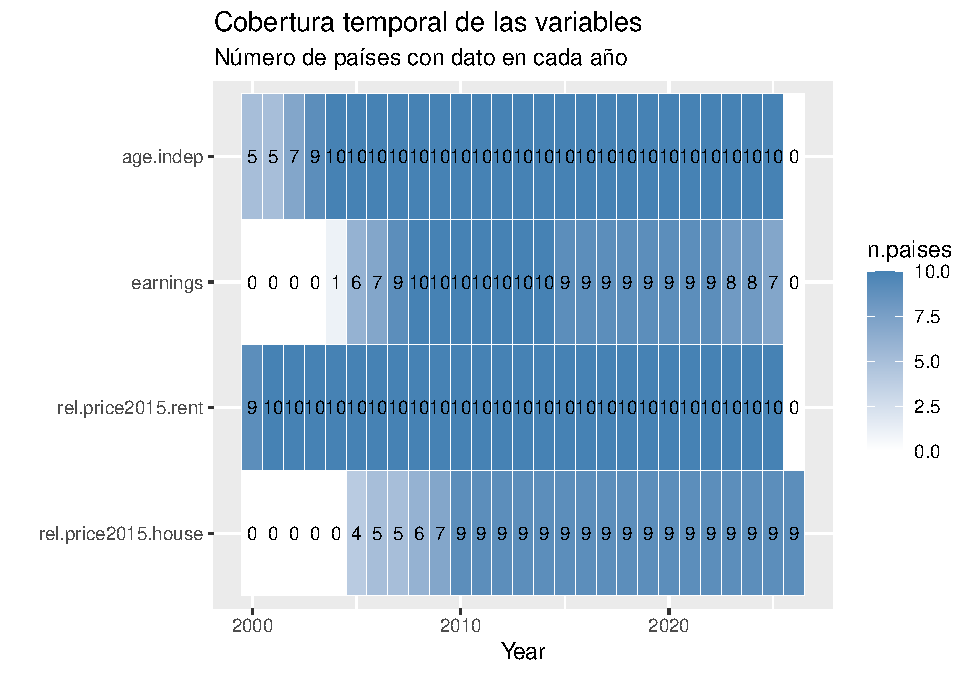
\includegraphics[keepaspectratio]{ProyectoAED_files/figure-latex/unnamed-chunk-9-1.pdf}}

\begin{Shaded}
\begin{Highlighting}[]
\FunctionTok{ggsave}\NormalTok{(}\StringTok{\textquotesingle{}results/univ\_cobertura.pdf\textquotesingle{}}\NormalTok{, }\AttributeTok{width =} \DecValTok{14}\NormalTok{, }\AttributeTok{height =} \DecValTok{10}\NormalTok{, }\AttributeTok{dpi =} \DecValTok{300}\NormalTok{)}
\end{Highlighting}
\end{Shaded}

\begin{Shaded}
\begin{Highlighting}[]
\CommentTok{\# Limitamos el estudio desde el 2010 hasta el 2025}
\NormalTok{jovenes.df }\SpecialCharTok{\%\textless{}\textgreater{}\%} \FunctionTok{filter}\NormalTok{(year }\SpecialCharTok{\textgreater{}=} \DecValTok{2010} \SpecialCharTok{\&}\NormalTok{ year }\SpecialCharTok{\textless{}=} \DecValTok{2025}\NormalTok{)}

\CommentTok{\# Obtenemos el primer año en el que comienzan las medidas de salarios y precios}
\CommentTok{\# Tomamos este año como valor de referencia para poder compararlos luego mas facilmente}
\NormalTok{year.start }\OtherTok{\textless{}{-}}\NormalTok{ jovenes.df }\SpecialCharTok{\%\textgreater{}\%} \FunctionTok{group\_by}\NormalTok{(country) }\SpecialCharTok{\%\textgreater{}\%} \FunctionTok{arrange}\NormalTok{(year) }\SpecialCharTok{\%\textgreater{}\%} \FunctionTok{select}\NormalTok{(}\FunctionTok{c}\NormalTok{(country, year, rel.price2015.rent, rel.price2015.house, earnings)) }\SpecialCharTok{\%\textgreater{}\%}  \FunctionTok{filter}\NormalTok{(}\FunctionTok{if\_all}\NormalTok{(}\FunctionTok{everything}\NormalTok{(), }\SpecialCharTok{\textasciitilde{}} \SpecialCharTok{!}\FunctionTok{is.na}\NormalTok{(.x))) }\SpecialCharTok{\%\textgreater{}\%} \FunctionTok{slice}\NormalTok{(}\DecValTok{1}\NormalTok{) }\SpecialCharTok{\%\textgreater{}\%} \FunctionTok{ungroup}\NormalTok{() }\SpecialCharTok{\%\textgreater{}\%} \FunctionTok{transmute}\NormalTok{(country, }\AttributeTok{year.start =}\NormalTok{ year)}

\NormalTok{jovenes.df }\OtherTok{\textless{}{-}} \FunctionTok{full\_join}\NormalTok{(jovenes.df, year.start)}
\end{Highlighting}
\end{Shaded}

\begin{verbatim}
## Joining with `by = join_by(country)`
\end{verbatim}

\begin{Shaded}
\begin{Highlighting}[]
\CommentTok{\# Ahora tomamos, para cada variable, un valor de 100 en el año de referencia, asi las podremos comparar mejor graficamente}
\NormalTok{jovenes.df }\SpecialCharTok{\%\textless{}\textgreater{}\%} \FunctionTok{group\_by}\NormalTok{(country) }\SpecialCharTok{\%\textgreater{}\%} \FunctionTok{mutate}\NormalTok{(}\AttributeTok{earnings =}\NormalTok{ earnings}\SpecialCharTok{/}\NormalTok{earnings[year }\SpecialCharTok{==} \FunctionTok{unique}\NormalTok{(year.start)]}\SpecialCharTok{*}\DecValTok{100}\NormalTok{, }\AttributeTok{price.rent =}\NormalTok{ rel.price2015.rent}\SpecialCharTok{/}\NormalTok{rel.price2015.rent[year }\SpecialCharTok{==} \FunctionTok{unique}\NormalTok{(year.start)]}\SpecialCharTok{*}\DecValTok{100}\NormalTok{, }\AttributeTok{price.house =}\NormalTok{ rel.price2015.house}\SpecialCharTok{/}\NormalTok{rel.price2015.house[year }\SpecialCharTok{==} \FunctionTok{unique}\NormalTok{(year.start)]}\SpecialCharTok{*}\DecValTok{100}\NormalTok{) }\SpecialCharTok{\%\textgreater{}\%} \FunctionTok{select}\NormalTok{(}\FunctionTok{c}\NormalTok{(}\SpecialCharTok{{-}}\NormalTok{year.start, }\SpecialCharTok{{-}}\NormalTok{rel.price2015.rent, }\SpecialCharTok{{-}}\NormalTok{rel.price2015.house)) }\SpecialCharTok{\%\textgreater{}\%} \FunctionTok{ungroup}\NormalTok{()}

\CommentTok{\# Calculamos los salarios en proporcion al precio de la vivienda y a los alquileres, respectivamente}
\NormalTok{jovenes.df }\SpecialCharTok{\%\textless{}\textgreater{}\%} \FunctionTok{mutate}\NormalTok{(}\AttributeTok{earn.prop.house =}\NormalTok{ earnings}\SpecialCharTok{/}\NormalTok{price.house}\SpecialCharTok{*}\DecValTok{100}\NormalTok{, }\AttributeTok{earn.prop.rent =}\NormalTok{ earnings}\SpecialCharTok{/}\NormalTok{price.rent}\SpecialCharTok{*}\DecValTok{100}\NormalTok{)}

\CommentTok{\# Calculamos el aumento porcentual de los salarios, alquileres y precio de la vivienda para cada año}
\NormalTok{jovenes.df }\SpecialCharTok{\%\textless{}\textgreater{}\%}
  \FunctionTok{group\_by}\NormalTok{(country) }\SpecialCharTok{\%\textgreater{}\%}
  \FunctionTok{arrange}\NormalTok{(year, }\AttributeTok{.by\_group =} \ConstantTok{TRUE}\NormalTok{) }\SpecialCharTok{\%\textgreater{}\%}
  \FunctionTok{mutate}\NormalTok{(}
    \AttributeTok{age.diff =}\NormalTok{ age.indep }\SpecialCharTok{{-}} \FunctionTok{lag}\NormalTok{(age.indep),}
    \AttributeTok{earn.diff =}\NormalTok{ earnings }\SpecialCharTok{{-}} \FunctionTok{lag}\NormalTok{(earnings),}
    \AttributeTok{house.diff =}\NormalTok{ price.house }\SpecialCharTok{{-}} \FunctionTok{lag}\NormalTok{(price.house),}
    \AttributeTok{rent.diff =}\NormalTok{ price.rent }\SpecialCharTok{{-}} \FunctionTok{lag}\NormalTok{(price.rent)}
\NormalTok{  ) }\SpecialCharTok{\%\textgreater{}\%}
  \FunctionTok{ungroup}\NormalTok{()}
\end{Highlighting}
\end{Shaded}

\begin{Shaded}
\begin{Highlighting}[]
\CommentTok{\# Calculamos ahora cuales son las variables cuantitativas continuas tras las transformaciones}
\NormalTok{vars.num }\OtherTok{\textless{}{-}} \FunctionTok{setdiff}\NormalTok{(}\FunctionTok{colnames}\NormalTok{(jovenes.df)[}\FunctionTok{sapply}\NormalTok{(jovenes.df, is.numeric)], }\StringTok{\textquotesingle{}year\textquotesingle{}}\NormalTok{)}
\NormalTok{vars.num}
\end{Highlighting}
\end{Shaded}

\begin{verbatim}
##  [1] "age.indep"       "earnings"        "price.rent"      "price.house"    
##  [5] "earn.prop.house" "earn.prop.rent"  "age.diff"        "earn.diff"      
##  [9] "house.diff"      "rent.diff"
\end{verbatim}

\section{Estudio de variables}\label{estudio-de-variables}

\begin{Shaded}
\begin{Highlighting}[]
\NormalTok{sumario.jovenes }\OtherTok{\textless{}{-}} \FunctionTok{data.frame}\NormalTok{(}\AttributeTok{variable =} \FunctionTok{colnames}\NormalTok{(jovenes.df))}
\NormalTok{sumario.jovenes}\SpecialCharTok{$}\NormalTok{type }\OtherTok{\textless{}{-}} \FunctionTok{sapply}\NormalTok{(jovenes.df, }\ControlFlowTok{function}\NormalTok{(x) }\FunctionTok{class}\NormalTok{(x)[}\DecValTok{1}\NormalTok{])}
\NormalTok{sumario.jovenes}\SpecialCharTok{$}\NormalTok{levels }\OtherTok{\textless{}{-}} \FunctionTok{sapply}\NormalTok{(jovenes.df, }\ControlFlowTok{function}\NormalTok{(x) }\FunctionTok{length}\NormalTok{(}\FunctionTok{unique}\NormalTok{(x)))}
\NormalTok{sumario.jovenes}\SpecialCharTok{$}\NormalTok{topLevel }\OtherTok{\textless{}{-}} \FunctionTok{sapply}\NormalTok{(jovenes.df, }\ControlFlowTok{function}\NormalTok{(x) }\FunctionTok{names}\NormalTok{(}\FunctionTok{which.max}\NormalTok{(}\FunctionTok{table}\NormalTok{(x))))}
\NormalTok{sumario.jovenes}\SpecialCharTok{$}\NormalTok{topCount }\OtherTok{\textless{}{-}} \FunctionTok{sapply}\NormalTok{(jovenes.df, }\ControlFlowTok{function}\NormalTok{(x) }\FunctionTok{max}\NormalTok{(}\FunctionTok{table}\NormalTok{(x)))}
\NormalTok{sumario.jovenes}\SpecialCharTok{$}\NormalTok{topFrac }\OtherTok{\textless{}{-}}\NormalTok{ sumario.jovenes}\SpecialCharTok{$}\NormalTok{topCount }\SpecialCharTok{/} \FunctionTok{nrow}\NormalTok{(jovenes.df)}
\NormalTok{sumario.jovenes}\SpecialCharTok{$}\NormalTok{missFreq }\OtherTok{\textless{}{-}} \FunctionTok{sapply}\NormalTok{(jovenes.df, }\ControlFlowTok{function}\NormalTok{(x) }\FunctionTok{sum}\NormalTok{(}\FunctionTok{is.na}\NormalTok{(x)))}
\NormalTok{sumario.jovenes}\SpecialCharTok{$}\NormalTok{missFrac }\OtherTok{\textless{}{-}}\NormalTok{ sumario.jovenes}\SpecialCharTok{$}\NormalTok{missFreq }\SpecialCharTok{/} \FunctionTok{nrow}\NormalTok{(jovenes.df)}

\NormalTok{sumario.jovenes}
\end{Highlighting}
\end{Shaded}

\begin{verbatim}
##           variable    type levels          topLevel topCount topFrac missFreq
## 1          country  factor     10                DE       16 0.10000        0
## 2             year numeric     16              2010       10 0.06250        0
## 3        age.indep numeric     61              23.7       12 0.07500        0
## 4         earnings numeric    128               100        9 0.05625       25
## 5       price.rent numeric    136               100        9 0.05625       16
## 6      price.house numeric    136               100        9 0.05625       16
## 7  earn.prop.house numeric    128               100        9 0.05625       25
## 8   earn.prop.rent numeric    128               100        9 0.05625       25
## 9         age.diff numeric     29                 0       31 0.19375       10
## 10       earn.diff numeric    127 -26.0178668438882        1 0.00625       34
## 11      house.diff numeric    134  1.45547945205479        3 0.01875       25
## 12       rent.diff numeric    132 0.210084033613441        2 0.01250       25
##    missFrac
## 1   0.00000
## 2   0.00000
## 3   0.00000
## 4   0.15625
## 5   0.10000
## 6   0.10000
## 7   0.15625
## 8   0.15625
## 9   0.06250
## 10  0.21250
## 11  0.15625
## 12  0.15625
\end{verbatim}

\begin{Shaded}
\begin{Highlighting}[]
\NormalTok{cobertura.var }\OtherTok{\textless{}{-}} \FunctionTok{data.frame}\NormalTok{(}\AttributeTok{variable =}\NormalTok{ vars.num)}
\NormalTok{cobertura.var}\SpecialCharTok{$}\NormalTok{year.min }\OtherTok{\textless{}{-}} \FunctionTok{unname}\NormalTok{(}\FunctionTok{sapply}\NormalTok{(vars.num, }\ControlFlowTok{function}\NormalTok{(v) }\FunctionTok{min}\NormalTok{(jovenes.df}\SpecialCharTok{$}\NormalTok{year[}\SpecialCharTok{!}\FunctionTok{is.na}\NormalTok{(jovenes.df[[v]])])))}
\NormalTok{cobertura.var}\SpecialCharTok{$}\NormalTok{year.max }\OtherTok{\textless{}{-}} \FunctionTok{unname}\NormalTok{(}\FunctionTok{sapply}\NormalTok{(vars.num, }\ControlFlowTok{function}\NormalTok{(v) }\FunctionTok{max}\NormalTok{(jovenes.df}\SpecialCharTok{$}\NormalTok{year[}\SpecialCharTok{!}\FunctionTok{is.na}\NormalTok{(jovenes.df[[v]])])))}
\NormalTok{cobertura.var}\SpecialCharTok{$}\NormalTok{n.obs }\OtherTok{\textless{}{-}} \FunctionTok{unname}\NormalTok{(}\FunctionTok{sapply}\NormalTok{(vars.num, }\ControlFlowTok{function}\NormalTok{(v) }\FunctionTok{sum}\NormalTok{(}\SpecialCharTok{!}\FunctionTok{is.na}\NormalTok{(jovenes.df[[v]]))))}
\NormalTok{cobertura.var}\SpecialCharTok{$}\NormalTok{n.paises }\OtherTok{\textless{}{-}} \FunctionTok{unname}\NormalTok{(}\FunctionTok{sapply}\NormalTok{(vars.num, }\ControlFlowTok{function}\NormalTok{(v) }\FunctionTok{length}\NormalTok{(}\FunctionTok{unique}\NormalTok{(jovenes.df}\SpecialCharTok{$}\NormalTok{country[}\SpecialCharTok{!}\FunctionTok{is.na}\NormalTok{(jovenes.df[[v]])]))))}
\NormalTok{cobertura.var}
\end{Highlighting}
\end{Shaded}

\begin{verbatim}
##           variable year.min year.max n.obs n.paises
## 1        age.indep     2010     2025   160       10
## 2         earnings     2010     2025   135        9
## 3       price.rent     2010     2025   144        9
## 4      price.house     2010     2025   144        9
## 5  earn.prop.house     2010     2025   135        9
## 6   earn.prop.rent     2010     2025   135        9
## 7         age.diff     2011     2025   150       10
## 8        earn.diff     2011     2025   126        9
## 9       house.diff     2011     2025   135        9
## 10       rent.diff     2011     2025   135        9
\end{verbatim}

\section{Análisis univariante}\label{anuxe1lisis-univariante}

\subsection{Estadísticos descriptivos de las variables
numéricas}\label{estaduxedsticos-descriptivos-de-las-variables-numuxe9ricas}

\begin{Shaded}
\begin{Highlighting}[]
\NormalTok{mystats }\OtherTok{\textless{}{-}} \ControlFlowTok{function}\NormalTok{(x, }\AttributeTok{na.omit =} \ConstantTok{TRUE}\NormalTok{) \{}
  \ControlFlowTok{if}\NormalTok{ (na.omit) x }\OtherTok{\textless{}{-}}\NormalTok{ x[}\SpecialCharTok{!}\FunctionTok{is.na}\NormalTok{(x)]}
\NormalTok{  m }\OtherTok{\textless{}{-}} \FunctionTok{mean}\NormalTok{(x)}
\NormalTok{  n }\OtherTok{\textless{}{-}} \FunctionTok{length}\NormalTok{(x)}
\NormalTok{  s }\OtherTok{\textless{}{-}} \FunctionTok{sd}\NormalTok{(x)}
\NormalTok{  skew }\OtherTok{\textless{}{-}} \FunctionTok{sum}\NormalTok{((x }\SpecialCharTok{{-}}\NormalTok{ m)}\SpecialCharTok{\^{}}\DecValTok{3} \SpecialCharTok{/}\NormalTok{ s}\SpecialCharTok{\^{}}\DecValTok{3}\NormalTok{) }\SpecialCharTok{/}\NormalTok{ n}
\NormalTok{  kurt }\OtherTok{\textless{}{-}} \FunctionTok{sum}\NormalTok{((x }\SpecialCharTok{{-}}\NormalTok{ m)}\SpecialCharTok{\^{}}\DecValTok{4} \SpecialCharTok{/}\NormalTok{ s}\SpecialCharTok{\^{}}\DecValTok{4}\NormalTok{) }\SpecialCharTok{/}\NormalTok{ n }\SpecialCharTok{{-}} \DecValTok{3}
  \FunctionTok{return}\NormalTok{(}\FunctionTok{c}\NormalTok{(}\AttributeTok{n =}\NormalTok{ n, }\AttributeTok{mean =}\NormalTok{ m, }\AttributeTok{trimmed =} \FunctionTok{mean}\NormalTok{(x, }\AttributeTok{trim =} \FloatTok{0.1}\NormalTok{), }\AttributeTok{median =} \FunctionTok{median}\NormalTok{(x), }\AttributeTok{min =} \FunctionTok{min}\NormalTok{(x), }\AttributeTok{q1 =} \FunctionTok{quantile}\NormalTok{(x, }\FloatTok{0.25}\NormalTok{, }\AttributeTok{names =} \ConstantTok{FALSE}\NormalTok{), }\AttributeTok{q3 =} \FunctionTok{quantile}\NormalTok{(x, }\FloatTok{0.75}\NormalTok{, }\AttributeTok{names =} \ConstantTok{FALSE}\NormalTok{), }\AttributeTok{max =} \FunctionTok{max}\NormalTok{(x), }\AttributeTok{stdev =}\NormalTok{ s, }\AttributeTok{var =} \FunctionTok{var}\NormalTok{(x), }\AttributeTok{mad =} \FunctionTok{mad}\NormalTok{(x), }\AttributeTok{IQR =} \FunctionTok{IQR}\NormalTok{(x), }\AttributeTok{skew =}\NormalTok{ skew, }\AttributeTok{kurtosis =}\NormalTok{ kurt))}
\NormalTok{\}}
\CommentTok{\# Funcion del Tema 6 (asimetria y curtosis en exceso), ampliada con media recortada (10\%), cuartiles, rango intercuartilico y MAD}

\NormalTok{estad }\OtherTok{\textless{}{-}} \FunctionTok{sapply}\NormalTok{(jovenes.df[vars.num], mystats)}

\FunctionTok{t}\NormalTok{(}\FunctionTok{round}\NormalTok{(estad[}\FunctionTok{c}\NormalTok{(}\StringTok{\textquotesingle{}n\textquotesingle{}}\NormalTok{, }\StringTok{\textquotesingle{}mean\textquotesingle{}}\NormalTok{, }\StringTok{\textquotesingle{}trimmed\textquotesingle{}}\NormalTok{, }\StringTok{\textquotesingle{}median\textquotesingle{}}\NormalTok{, }\StringTok{\textquotesingle{}min\textquotesingle{}}\NormalTok{, }\StringTok{\textquotesingle{}q1\textquotesingle{}}\NormalTok{, }\StringTok{\textquotesingle{}q3\textquotesingle{}}\NormalTok{, }\StringTok{\textquotesingle{}max\textquotesingle{}}\NormalTok{), ], }\DecValTok{2}\NormalTok{))}
\end{Highlighting}
\end{Shaded}

\begin{verbatim}
##                   n   mean trimmed median    min     q1     q3    max
## age.indep       160  26.77   26.74  27.00  23.00  23.90  29.00  30.90
## earnings        135 121.47  109.75 103.22  64.26  95.58 118.49 431.60
## price.rent      144 115.02  111.73 108.71  99.46 104.36 118.98 190.88
## price.house     144 116.87  111.63 106.05  71.00  94.69 130.36 247.48
## earn.prop.house 135 106.72   98.67 100.00  63.85  83.69 112.76 330.68
## earn.prop.rent  135 103.76   96.97  97.48  64.35  86.01 105.86 258.22
## age.diff        150   0.02    0.02   0.00  -1.80  -0.10   0.20   1.80
## earn.diff       126   6.04    3.72   4.08 -26.02  -3.03  10.20  64.47
## house.diff      135   4.20    3.71   3.47 -13.68   0.46   6.87  43.17
## rent.diff       135   2.86    2.23   1.81  -1.30   1.15   3.17  19.45
\end{verbatim}

\begin{Shaded}
\begin{Highlighting}[]
\CommentTok{\# Tendencia central y posicion}

\FunctionTok{t}\NormalTok{(}\FunctionTok{round}\NormalTok{(estad[}\FunctionTok{c}\NormalTok{(}\StringTok{\textquotesingle{}stdev\textquotesingle{}}\NormalTok{, }\StringTok{\textquotesingle{}var\textquotesingle{}}\NormalTok{, }\StringTok{\textquotesingle{}mad\textquotesingle{}}\NormalTok{, }\StringTok{\textquotesingle{}IQR\textquotesingle{}}\NormalTok{, }\StringTok{\textquotesingle{}skew\textquotesingle{}}\NormalTok{, }\StringTok{\textquotesingle{}kurtosis\textquotesingle{}}\NormalTok{), ], }\DecValTok{2}\NormalTok{))}
\end{Highlighting}
\end{Shaded}

\begin{verbatim}
##                 stdev     var   mad   IQR  skew kurtosis
## age.indep        2.49    6.21  3.56  5.10 -0.03    -1.48
## earnings        55.57 3087.57 15.46 22.91  3.03    10.57
## price.rent      17.18  295.04  8.92 14.62  2.06     4.55
## price.house     34.21 1170.42 22.36 35.67  1.48     2.01
## earn.prop.house 42.96 1845.74 22.56 29.07  3.11    10.71
## earn.prop.rent  33.83 1144.40 15.12 19.85  2.74     8.00
## age.diff         0.35    0.12  0.30  0.30 -0.18     8.67
## earn.diff       16.95  287.13  9.41 13.24  1.68     3.61
## house.diff       7.66   58.70  4.87  6.41  1.35     5.13
## rent.diff        3.31   10.96  1.31  2.02  2.63     8.27
\end{verbatim}

\begin{Shaded}
\begin{Highlighting}[]
\CommentTok{\# Dispersion y forma (skew \textgreater{} 0: cola larga a la derecha; kurtosis \textgreater{} 0: colas mas pesadas que la normal)}
\end{Highlighting}
\end{Shaded}

\subsection{Edad de emancipación}\label{edad-de-emancipaciuxf3n}

\begin{Shaded}
\begin{Highlighting}[]
\NormalTok{age.mean }\OtherTok{\textless{}{-}}\NormalTok{ jovenes.df }\SpecialCharTok{\%\textgreater{}\%} \FunctionTok{group\_by}\NormalTok{(year) }\SpecialCharTok{\%\textgreater{}\%} \FunctionTok{summarise}\NormalTok{(}\AttributeTok{age.mean =} \FunctionTok{mean}\NormalTok{(age.indep, }\AttributeTok{na.rm =} \ConstantTok{TRUE}\NormalTok{), }\AttributeTok{.groups =} \StringTok{"drop"}\NormalTok{)}
\FunctionTok{ggplot}\NormalTok{() }\SpecialCharTok{+} \FunctionTok{geom\_line}\NormalTok{(}\AttributeTok{data =}\NormalTok{ jovenes.df, }\AttributeTok{mapping =} \FunctionTok{aes}\NormalTok{(}\AttributeTok{x =}\NormalTok{ year, }\AttributeTok{y =}\NormalTok{ age.indep, }\AttributeTok{color =}\NormalTok{ country), }\AttributeTok{linewidth =} \FloatTok{1.15}\NormalTok{, }\AttributeTok{na.rm =} \ConstantTok{TRUE}\NormalTok{) }\SpecialCharTok{+} \FunctionTok{geom\_line}\NormalTok{(}\AttributeTok{data =}\NormalTok{ age.mean, }\AttributeTok{mapping =} \FunctionTok{aes}\NormalTok{(}\AttributeTok{x =}\NormalTok{ year, }\AttributeTok{y =}\NormalTok{ age.mean, }\AttributeTok{color =} \StringTok{\textquotesingle{}mean\textquotesingle{}}\NormalTok{), }\AttributeTok{linewidth =} \FloatTok{1.15}\NormalTok{, }\AttributeTok{na.rm =} \ConstantTok{TRUE}\NormalTok{) }\SpecialCharTok{+}
  \FunctionTok{scale\_color\_manual}\NormalTok{(}\AttributeTok{values =} \FunctionTok{c}\NormalTok{(}\FunctionTok{setNames}\NormalTok{(scales}\SpecialCharTok{::}\FunctionTok{hue\_pal}\NormalTok{()(}\FunctionTok{length}\NormalTok{(}\FunctionTok{unique}\NormalTok{(jovenes.df}\SpecialCharTok{$}\NormalTok{country))), }\FunctionTok{unique}\NormalTok{(jovenes.df}\SpecialCharTok{$}\NormalTok{country)), }\StringTok{"mean"} \OtherTok{=} \StringTok{"black"}\NormalTok{)) }\SpecialCharTok{+}
  \FunctionTok{labs}\NormalTok{(}\AttributeTok{title =} \StringTok{\textquotesingle{}Evolución temporal de la edad de emancipación\textquotesingle{}}\NormalTok{) }\SpecialCharTok{+} \FunctionTok{xlab}\NormalTok{(}\StringTok{\textquotesingle{}Year\textquotesingle{}}\NormalTok{) }\SpecialCharTok{+} \FunctionTok{ylab}\NormalTok{(}\StringTok{\textquotesingle{}Age\textquotesingle{}}\NormalTok{)}
\end{Highlighting}
\end{Shaded}

\pandocbounded{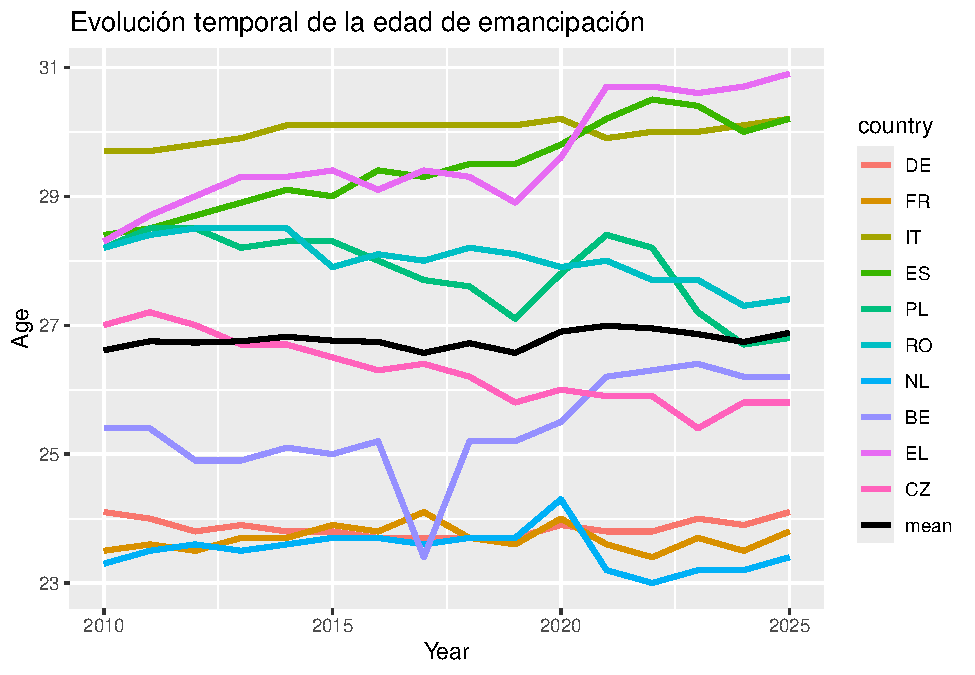
\includegraphics[keepaspectratio]{ProyectoAED_files/figure-latex/unnamed-chunk-15-1.pdf}}

\begin{Shaded}
\begin{Highlighting}[]
\FunctionTok{ggsave}\NormalTok{(}\StringTok{\textquotesingle{}results/edad\_emancipacion.pdf\textquotesingle{}}\NormalTok{, }\AttributeTok{width =} \DecValTok{14}\NormalTok{, }\AttributeTok{height =} \DecValTok{10}\NormalTok{, }\AttributeTok{dpi =} \DecValTok{300}\NormalTok{)}
\end{Highlighting}
\end{Shaded}

\begin{Shaded}
\begin{Highlighting}[]
\NormalTok{media.edad }\OtherTok{\textless{}{-}}\NormalTok{ jovenes.df }\SpecialCharTok{\%\textgreater{}\%} \FunctionTok{group\_by}\NormalTok{(country) }\SpecialCharTok{\%\textgreater{}\%} \FunctionTok{summarise}\NormalTok{(}\AttributeTok{n.years =} \FunctionTok{n}\NormalTok{(), }\AttributeTok{media =} \FunctionTok{round}\NormalTok{(}\FunctionTok{mean}\NormalTok{(age.indep, }\AttributeTok{na.rm =} \ConstantTok{TRUE}\NormalTok{),}\DecValTok{2}\NormalTok{), }\AttributeTok{media.pct =} \FunctionTok{round}\NormalTok{(}\FunctionTok{mean}\NormalTok{(age.diff, }\AttributeTok{na.rm =} \ConstantTok{TRUE}\NormalTok{),}\DecValTok{2}\NormalTok{), }\AttributeTok{total.dif =}\NormalTok{ age.indep[}\FunctionTok{length}\NormalTok{(age.indep)]}\SpecialCharTok{{-}}\NormalTok{age.indep[}\DecValTok{1}\NormalTok{], }\AttributeTok{.groups =} \StringTok{\textquotesingle{}drop\textquotesingle{}}\NormalTok{) }\SpecialCharTok{\%\textgreater{}\%} \FunctionTok{as.data.frame}\NormalTok{()}
\NormalTok{media.edad}
\end{Highlighting}
\end{Shaded}

\begin{verbatim}
##    country n.years media media.pct total.dif
## 1       DE      16 23.86      0.00       0.0
## 2       FR      16 23.69      0.02       0.3
## 3       IT      16 30.01      0.03       0.5
## 4       ES      16 29.46      0.12       1.8
## 5       PL      16 27.84     -0.09      -1.4
## 6       RO      16 28.02     -0.05      -0.8
## 7       NL      16 23.51      0.01       0.1
## 8       BE      16 25.41      0.05       0.8
## 9       EL      16 29.62      0.17       2.6
## 10      CZ      16 26.29     -0.08      -1.2
\end{verbatim}

\begin{Shaded}
\begin{Highlighting}[]
\CommentTok{\# Media anual de cada pais de la edad de emancipación}
\end{Highlighting}
\end{Shaded}

\subsection{Media del aumento anual por país: salarios, alquiler y
vivienda}\label{media-del-aumento-anual-por-pauxeds-salarios-alquiler-y-vivienda}

\begin{verbatim}
## year.ini year.fin 
##     2010     2020
\end{verbatim}

\begin{verbatim}
##   country  n
## 1      DE 10
## 2      FR 10
## 3      IT 10
## 4      ES 10
## 5      PL 10
## 6      RO 10
## 7      NL 10
## 8      BE 10
## 9      CZ 10
\end{verbatim}

\begin{Shaded}
\begin{Highlighting}[]
\NormalTok{jovenes.df }\SpecialCharTok{\%\textgreater{}\%} \FunctionTok{filter}\NormalTok{(country }\SpecialCharTok{\%in\%}\NormalTok{ mas.poblacion5) }\SpecialCharTok{\%\textgreater{}\%} \FunctionTok{ggplot}\NormalTok{(}\FunctionTok{aes}\NormalTok{(}\AttributeTok{x=}\NormalTok{earn.diff)) }\SpecialCharTok{+}  \FunctionTok{geom\_histogram}\NormalTok{(}\AttributeTok{bins =} \DecValTok{30}\NormalTok{, }\AttributeTok{na.rm =} \ConstantTok{TRUE}\NormalTok{) }\SpecialCharTok{+} \FunctionTok{facet\_wrap}\NormalTok{(}\SpecialCharTok{\textasciitilde{}}\NormalTok{country, }\AttributeTok{nrow =} \DecValTok{3}\NormalTok{)}\SpecialCharTok{+} \FunctionTok{xlab}\NormalTok{(}\StringTok{\textquotesingle{}Earnings percentage increase (\%)\textquotesingle{}}\NormalTok{) }\SpecialCharTok{+} \FunctionTok{ylab}\NormalTok{(}\StringTok{\textquotesingle{}Frequency\textquotesingle{}}\NormalTok{) }\SpecialCharTok{+} \FunctionTok{labs}\NormalTok{(}\AttributeTok{title =} \StringTok{\textquotesingle{}Histograma de los incrementos anuales de los salarios\textquotesingle{}}\NormalTok{, }\AttributeTok{subtitle =} \StringTok{\textquotesingle{}Por países\textquotesingle{}}\NormalTok{)}
\end{Highlighting}
\end{Shaded}

\pandocbounded{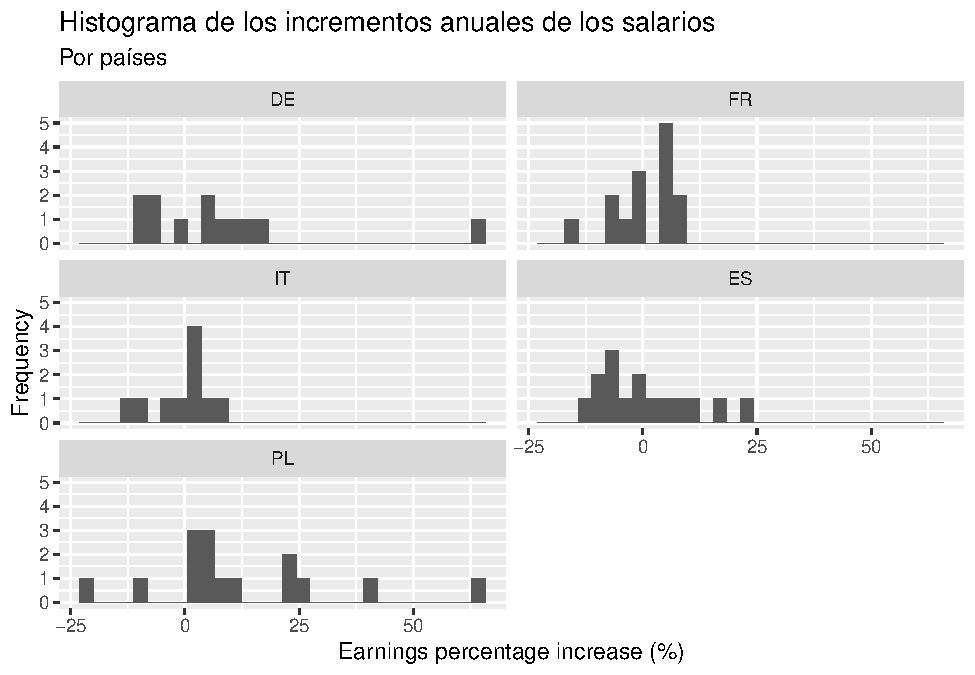
\includegraphics[keepaspectratio]{ProyectoAED_files/figure-latex/unnamed-chunk-18-1.pdf}}

\begin{Shaded}
\begin{Highlighting}[]
\NormalTok{jovenes.df }\SpecialCharTok{\%\textgreater{}\%} \FunctionTok{filter}\NormalTok{(country }\SpecialCharTok{\%in\%}\NormalTok{ mas.poblacion5) }\SpecialCharTok{\%\textgreater{}\%} \FunctionTok{ggplot}\NormalTok{(}\FunctionTok{aes}\NormalTok{(}\AttributeTok{x=}\NormalTok{house.diff)) }\SpecialCharTok{+}  \FunctionTok{geom\_histogram}\NormalTok{(}\AttributeTok{bins =} \DecValTok{30}\NormalTok{, }\AttributeTok{na.rm =} \ConstantTok{TRUE}\NormalTok{) }\SpecialCharTok{+} \FunctionTok{facet\_wrap}\NormalTok{(}\SpecialCharTok{\textasciitilde{}}\NormalTok{country, }\AttributeTok{nrow =} \DecValTok{3}\NormalTok{)}\SpecialCharTok{+} \FunctionTok{xlab}\NormalTok{(}\StringTok{\textquotesingle{}House price percentage increase (\%)\textquotesingle{}}\NormalTok{) }\SpecialCharTok{+} \FunctionTok{ylab}\NormalTok{(}\StringTok{\textquotesingle{}Frequency\textquotesingle{}}\NormalTok{) }\SpecialCharTok{+} \FunctionTok{labs}\NormalTok{(}\AttributeTok{title =} \StringTok{\textquotesingle{}Histograma de los incrementos anuales del precio de la vivienda\textquotesingle{}}\NormalTok{, }\AttributeTok{subtitle =} \StringTok{\textquotesingle{}Por países\textquotesingle{}}\NormalTok{)}
\end{Highlighting}
\end{Shaded}

\pandocbounded{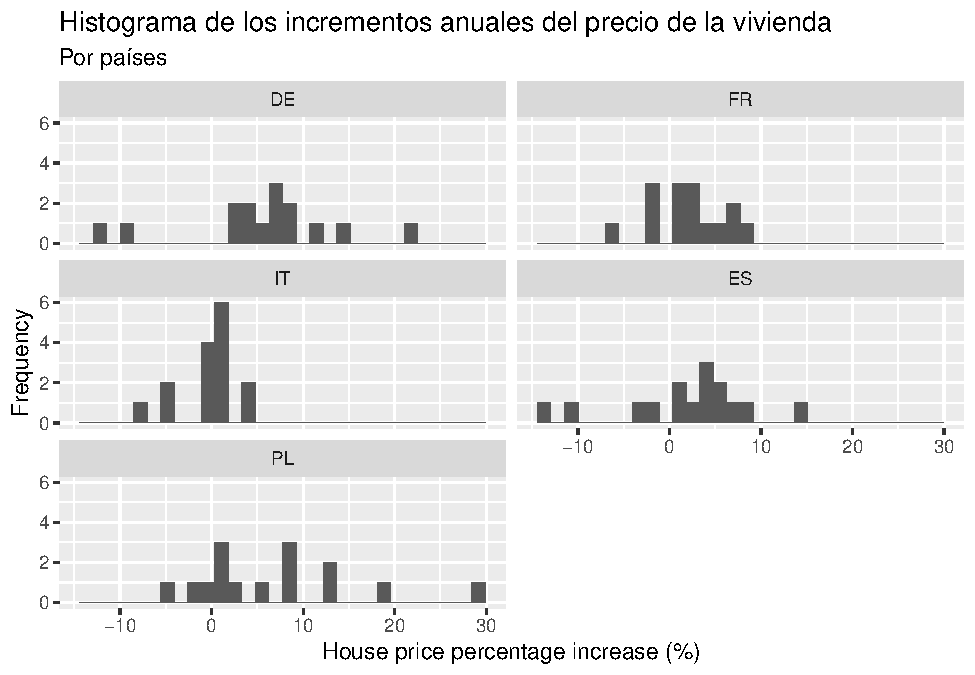
\includegraphics[keepaspectratio]{ProyectoAED_files/figure-latex/unnamed-chunk-19-1.pdf}}

\begin{Shaded}
\begin{Highlighting}[]
\NormalTok{jovenes.df }\SpecialCharTok{\%\textgreater{}\%} \FunctionTok{filter}\NormalTok{(country }\SpecialCharTok{\%in\%}\NormalTok{ mas.poblacion5) }\SpecialCharTok{\%\textgreater{}\%} \FunctionTok{ggplot}\NormalTok{(}\FunctionTok{aes}\NormalTok{(}\AttributeTok{x=}\NormalTok{rent.diff)) }\SpecialCharTok{+}  \FunctionTok{geom\_histogram}\NormalTok{(}\AttributeTok{bins =} \DecValTok{30}\NormalTok{, }\AttributeTok{na.rm =} \ConstantTok{TRUE}\NormalTok{) }\SpecialCharTok{+} \FunctionTok{facet\_wrap}\NormalTok{(}\SpecialCharTok{\textasciitilde{}}\NormalTok{country, }\AttributeTok{nrow =} \DecValTok{3}\NormalTok{)}\SpecialCharTok{+} \FunctionTok{xlab}\NormalTok{(}\StringTok{\textquotesingle{}Rent percentage increase (\%)\textquotesingle{}}\NormalTok{) }\SpecialCharTok{+} \FunctionTok{ylab}\NormalTok{(}\StringTok{\textquotesingle{}Frequency\textquotesingle{}}\NormalTok{) }\SpecialCharTok{+} \FunctionTok{labs}\NormalTok{(}\AttributeTok{title =} \StringTok{\textquotesingle{}Histograma de los incrementos anuales del alquiler\textquotesingle{}}\NormalTok{, }\AttributeTok{subtitle =} \StringTok{\textquotesingle{}Por países\textquotesingle{}}\NormalTok{)}
\end{Highlighting}
\end{Shaded}

\pandocbounded{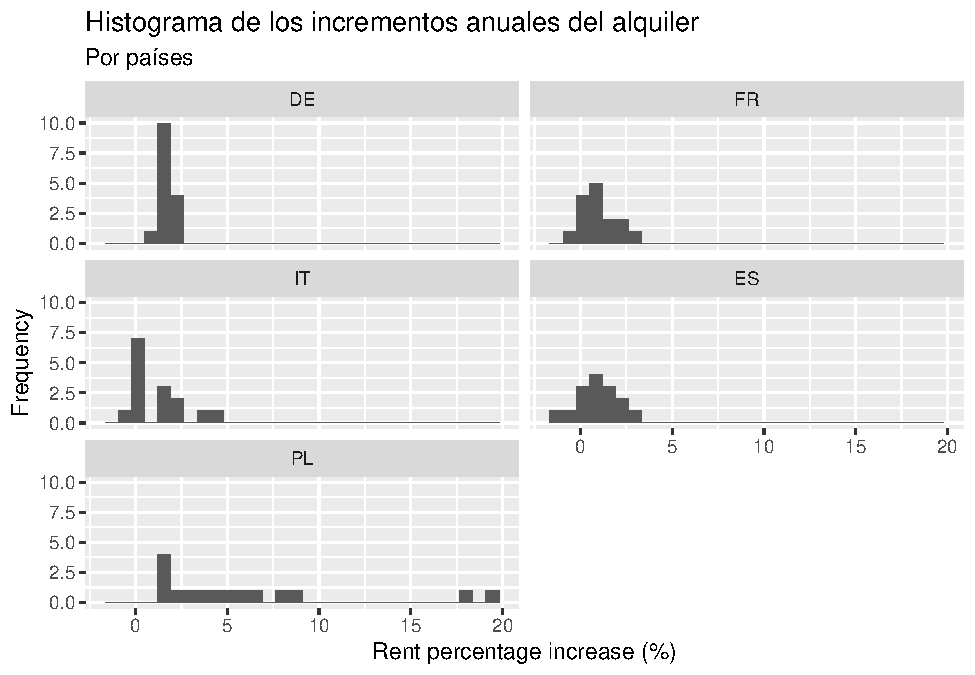
\includegraphics[keepaspectratio]{ProyectoAED_files/figure-latex/unnamed-chunk-20-1.pdf}}

\begin{Shaded}
\begin{Highlighting}[]
\NormalTok{medias.pais }\OtherTok{\textless{}{-}}\NormalTok{ aum.comun }\SpecialCharTok{\%\textgreater{}\%} \FunctionTok{group\_by}\NormalTok{(country) }\SpecialCharTok{\%\textgreater{}\%} \FunctionTok{summarise}\NormalTok{(}\AttributeTok{n.years =} \FunctionTok{n}\NormalTok{(), }\FunctionTok{across}\NormalTok{(}\FunctionTok{all\_of}\NormalTok{(vars.pct), mean), }\AttributeTok{.groups =} \StringTok{\textquotesingle{}drop\textquotesingle{}}\NormalTok{) }\SpecialCharTok{\%\textgreater{}\%} \FunctionTok{mutate}\NormalTok{(}\AttributeTok{earn.menos.house =}\NormalTok{ earn.pct }\SpecialCharTok{{-}}\NormalTok{ house.pct, }\AttributeTok{earn.menos.rent =}\NormalTok{ earn.pct }\SpecialCharTok{{-}}\NormalTok{ rent.pct) }\SpecialCharTok{\%\textgreater{}\%} \FunctionTok{as.data.frame}\NormalTok{()}
\NormalTok{medias.pais }\SpecialCharTok{\%\textgreater{}\%} \FunctionTok{mutate}\NormalTok{(}\FunctionTok{across}\NormalTok{(}\SpecialCharTok{{-}}\FunctionTok{c}\NormalTok{(country, n.years), }\SpecialCharTok{\textasciitilde{}} \FunctionTok{round}\NormalTok{(.x, }\DecValTok{2}\NormalTok{)))}
\end{Highlighting}
\end{Shaded}

\begin{verbatim}
##   country n.years house.pct rent.pct earn.pct earn.menos.house earn.menos.rent
## 1      DE      10      6.12     1.47     8.28             2.16            6.81
## 2      FR      10      1.78     0.73    -0.09            -1.87           -0.83
## 3      IT      10     -1.49     0.65    -0.34             1.15           -0.99
## 4      ES      10     -0.53     0.39    -1.13            -0.60           -1.52
## 5      PL      10      2.59     3.15     6.69             4.10            3.53
## 6      RO      10      0.46     1.76    13.49            13.04           11.73
## 7      NL      10      2.47     2.99     0.13            -2.35           -2.87
## 8      BE      10      2.79     1.44     0.31            -2.48           -1.13
## 9      CZ      10      5.65     2.66     4.36            -1.29            1.70
\end{verbatim}

\begin{Shaded}
\begin{Highlighting}[]
\CommentTok{\# Media anual de cada pais en la ventana comun y diferencias entre variables}
\end{Highlighting}
\end{Shaded}

\begin{Shaded}
\begin{Highlighting}[]
\NormalTok{pares }\OtherTok{\textless{}{-}} \FunctionTok{list}\NormalTok{(}\FunctionTok{c}\NormalTok{(}\StringTok{\textquotesingle{}earn.pct\textquotesingle{}}\NormalTok{, }\StringTok{\textquotesingle{}house.pct\textquotesingle{}}\NormalTok{), }\FunctionTok{c}\NormalTok{(}\StringTok{\textquotesingle{}earn.pct\textquotesingle{}}\NormalTok{, }\StringTok{\textquotesingle{}rent.pct\textquotesingle{}}\NormalTok{))}

\FunctionTok{data.frame}\NormalTok{(}\AttributeTok{par =} \FunctionTok{sapply}\NormalTok{(pares, paste, }\AttributeTok{collapse =} \StringTok{\textquotesingle{} vs \textquotesingle{}}\NormalTok{), }\AttributeTok{paises.mayor =} \FunctionTok{sapply}\NormalTok{(pares, }\ControlFlowTok{function}\NormalTok{(p) }\FunctionTok{sum}\NormalTok{(medias.pais[[p[}\DecValTok{1}\NormalTok{]]] }\SpecialCharTok{\textgreater{}}\NormalTok{ medias.pais[[p[}\DecValTok{2}\NormalTok{]]])), }\AttributeTok{n.paises =} \FunctionTok{nrow}\NormalTok{(medias.pais))}
\end{Highlighting}
\end{Shaded}

\begin{verbatim}
##                     par paises.mayor n.paises
## 1 earn.pct vs house.pct            4        9
## 2  earn.pct vs rent.pct            4        9
\end{verbatim}

\begin{Shaded}
\begin{Highlighting}[]
\CommentTok{\# paises.mayor: numero de paises en los que la media de la primera variable es mayor que la de la segunda}
\end{Highlighting}
\end{Shaded}

\section{Análisis bivariante}\label{anuxe1lisis-bivariante}

\begin{Shaded}
\begin{Highlighting}[]
\NormalTok{jovenes.df }\SpecialCharTok{\%\textgreater{}\%} \FunctionTok{filter}\NormalTok{(country }\SpecialCharTok{!=} \StringTok{\textquotesingle{}EL\textquotesingle{}}\NormalTok{) }\SpecialCharTok{\%\textgreater{}\%} \FunctionTok{ggplot}\NormalTok{(}\FunctionTok{aes}\NormalTok{(}\AttributeTok{x =}\NormalTok{ house.diff, }\AttributeTok{y =}\NormalTok{ earn.diff)) }\SpecialCharTok{+} \FunctionTok{geom\_point}\NormalTok{(}\AttributeTok{na.rm =} \ConstantTok{TRUE}\NormalTok{) }\SpecialCharTok{+} 
   \FunctionTok{geom\_smooth}\NormalTok{(}\AttributeTok{method =} \StringTok{"lm"}\NormalTok{, }\AttributeTok{se =} \ConstantTok{FALSE}\NormalTok{, }\AttributeTok{na.rm =} \ConstantTok{TRUE}\NormalTok{) }\SpecialCharTok{+} \FunctionTok{facet\_wrap}\NormalTok{(.}\SpecialCharTok{\textasciitilde{}}\NormalTok{country, }\AttributeTok{nrow =} \DecValTok{4}\NormalTok{, }\AttributeTok{scales =} \StringTok{\textquotesingle{}free\textquotesingle{}}\NormalTok{) }\SpecialCharTok{+} \FunctionTok{ylab}\NormalTok{(}\StringTok{\textquotesingle{}Earnings percentage increase (\%)\textquotesingle{}}\NormalTok{) }\SpecialCharTok{+} \FunctionTok{xlab}\NormalTok{(}\StringTok{\textquotesingle{}Housing price percentage increase (\%)\textquotesingle{}}\NormalTok{) }\SpecialCharTok{+} \FunctionTok{labs}\NormalTok{(}\AttributeTok{title =} \StringTok{\textquotesingle{}Salario de los jóvenes frente a precio de la vivienda\textquotesingle{}}\NormalTok{, }\AttributeTok{subtitle =} \StringTok{\textquotesingle{}En función de países\textquotesingle{}}\NormalTok{)}
\end{Highlighting}
\end{Shaded}

\pandocbounded{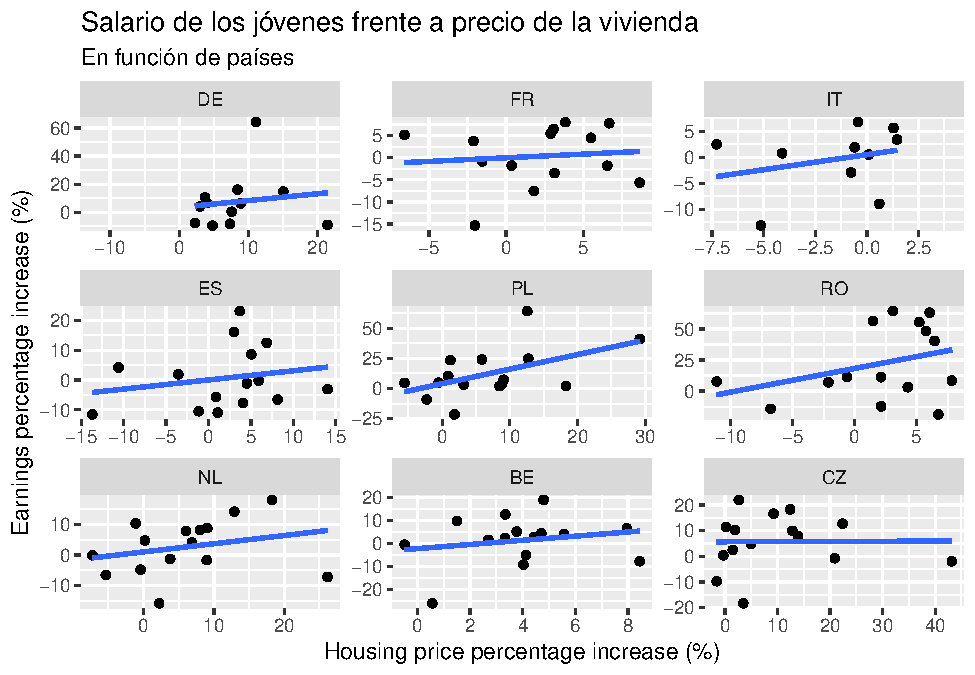
\includegraphics[keepaspectratio]{ProyectoAED_files/figure-latex/unnamed-chunk-23-1.pdf}}

\begin{Shaded}
\begin{Highlighting}[]
\NormalTok{jovenes.df }\SpecialCharTok{\%\textgreater{}\%} \FunctionTok{filter}\NormalTok{(country }\SpecialCharTok{!=} \StringTok{\textquotesingle{}EL\textquotesingle{}}\NormalTok{) }\SpecialCharTok{\%\textgreater{}\%} \FunctionTok{group\_by}\NormalTok{(country) }\SpecialCharTok{\%\textgreater{}\%} \FunctionTok{summarise}\NormalTok{(}\AttributeTok{cor.pearson =} \FunctionTok{cor}\NormalTok{(earn.diff, house.diff, }\AttributeTok{method =} \StringTok{\textquotesingle{}pearson\textquotesingle{}}\NormalTok{, }\AttributeTok{use =} \StringTok{\textquotesingle{}complete.obs\textquotesingle{}}\NormalTok{), }\AttributeTok{cor.spearman =} \FunctionTok{cor}\NormalTok{(earn.diff, house.diff, }\AttributeTok{method =} \StringTok{\textquotesingle{}spearman\textquotesingle{}}\NormalTok{, }\AttributeTok{use =} \StringTok{\textquotesingle{}complete.obs\textquotesingle{}}\NormalTok{))}
\end{Highlighting}
\end{Shaded}

\begin{verbatim}
## # A tibble: 9 x 3
##   country cor.pearson cor.spearman
##   <fct>         <dbl>        <dbl>
## 1 DE          0.136          0.217
## 2 FR          0.101          0.134
## 3 IT          0.272          0.345
## 4 ES          0.206          0.232
## 5 PL          0.517          0.386
## 6 RO          0.344          0.175
## 7 NL          0.260          0.3  
## 8 BE          0.205          0.207
## 9 CZ          0.00748        0.104
\end{verbatim}

\begin{Shaded}
\begin{Highlighting}[]
\NormalTok{jovenes.df }\SpecialCharTok{\%\textgreater{}\%} \FunctionTok{filter}\NormalTok{(country }\SpecialCharTok{!=} \StringTok{\textquotesingle{}EL\textquotesingle{}}\NormalTok{) }\SpecialCharTok{\%\textgreater{}\%} \FunctionTok{group\_by}\NormalTok{(country) }\SpecialCharTok{\%\textgreater{}\%} \FunctionTok{summarise}\NormalTok{(}\AttributeTok{slope =} \FunctionTok{lm}\NormalTok{(earn.diff }\SpecialCharTok{\textasciitilde{}}\NormalTok{ house.diff)[[}\DecValTok{1}\NormalTok{]][}\DecValTok{2}\NormalTok{])}
\end{Highlighting}
\end{Shaded}

\begin{verbatim}
## # A tibble: 9 x 2
##   country   slope
##   <fct>     <dbl>
## 1 DE      0.489  
## 2 FR      0.164  
## 3 IT      0.579  
## 4 ES      0.307  
## 5 PL      1.21   
## 6 RO      1.91   
## 7 NL      0.270  
## 8 BE      0.905  
## 9 CZ      0.00674
\end{verbatim}

\begin{Shaded}
\begin{Highlighting}[]
\NormalTok{jovenes.df }\SpecialCharTok{\%\textgreater{}\%} \FunctionTok{filter}\NormalTok{(country }\SpecialCharTok{!=} \StringTok{\textquotesingle{}EL\textquotesingle{}}\NormalTok{) }\SpecialCharTok{\%\textgreater{}\%} \FunctionTok{ggplot}\NormalTok{(}\FunctionTok{aes}\NormalTok{(}\AttributeTok{x =}\NormalTok{ rent.diff, }\AttributeTok{y =}\NormalTok{ earn.diff)) }\SpecialCharTok{+} \FunctionTok{geom\_point}\NormalTok{(}\AttributeTok{na.rm =} \ConstantTok{TRUE}\NormalTok{) }\SpecialCharTok{+} 
  \FunctionTok{geom\_smooth}\NormalTok{(}\AttributeTok{method =} \StringTok{"lm"}\NormalTok{, }\AttributeTok{se =} \ConstantTok{FALSE}\NormalTok{, }\AttributeTok{na.rm =} \ConstantTok{TRUE}\NormalTok{) }\SpecialCharTok{+} \FunctionTok{facet\_wrap}\NormalTok{(.}\SpecialCharTok{\textasciitilde{}}\NormalTok{country, }\AttributeTok{nrow =} \DecValTok{4}\NormalTok{, }\AttributeTok{scales =} \StringTok{\textquotesingle{}free\textquotesingle{}}\NormalTok{) }\SpecialCharTok{+} \FunctionTok{ylab}\NormalTok{(}\StringTok{\textquotesingle{}Earnings percentage increase (\%)\textquotesingle{}}\NormalTok{) }\SpecialCharTok{+} \FunctionTok{xlab}\NormalTok{(}\StringTok{\textquotesingle{}Rent percentage increase (\%)\textquotesingle{}}\NormalTok{) }\SpecialCharTok{+} \FunctionTok{labs}\NormalTok{(}\AttributeTok{title =} \StringTok{\textquotesingle{}Salario de los jóvenes frente a precio del alquiler\textquotesingle{}}\NormalTok{, }\AttributeTok{subtitle =} \StringTok{\textquotesingle{}En función de países\textquotesingle{}}\NormalTok{)}
\end{Highlighting}
\end{Shaded}

\pandocbounded{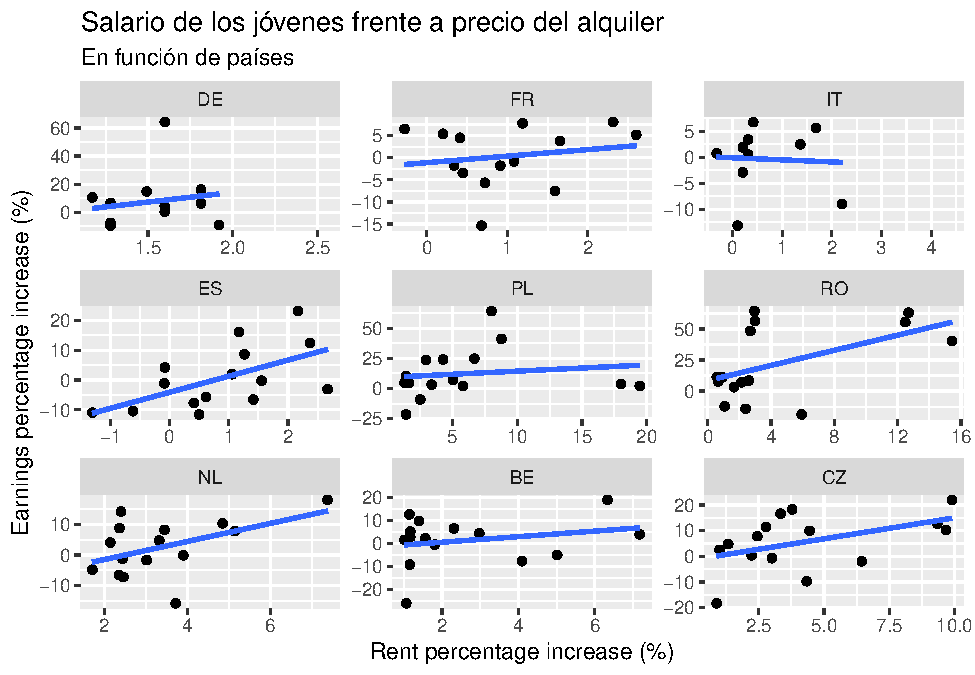
\includegraphics[keepaspectratio]{ProyectoAED_files/figure-latex/unnamed-chunk-26-1.pdf}}

\begin{Shaded}
\begin{Highlighting}[]
\NormalTok{jovenes.df }\SpecialCharTok{\%\textgreater{}\%} \FunctionTok{filter}\NormalTok{(country }\SpecialCharTok{!=} \StringTok{\textquotesingle{}EL\textquotesingle{}}\NormalTok{) }\SpecialCharTok{\%\textgreater{}\%} \FunctionTok{group\_by}\NormalTok{(country) }\SpecialCharTok{\%\textgreater{}\%} \FunctionTok{summarise}\NormalTok{(}\AttributeTok{cor.pearson =} \FunctionTok{cor}\NormalTok{(earn.diff, rent.diff, }\AttributeTok{method =} \StringTok{\textquotesingle{}pearson\textquotesingle{}}\NormalTok{, }\AttributeTok{use =} \StringTok{\textquotesingle{}complete.obs\textquotesingle{}}\NormalTok{), }\AttributeTok{cor.spearman =} \FunctionTok{cor}\NormalTok{(earn.diff, rent.diff, }\AttributeTok{method =} \StringTok{\textquotesingle{}spearman\textquotesingle{}}\NormalTok{, }\AttributeTok{use =} \StringTok{\textquotesingle{}complete.obs\textquotesingle{}}\NormalTok{))}
\end{Highlighting}
\end{Shaded}

\begin{verbatim}
## # A tibble: 9 x 3
##   country cor.pearson cor.spearman
##   <fct>         <dbl>        <dbl>
## 1 DE           0.174        0.154 
## 2 FR           0.178        0.0901
## 3 IT          -0.0514       0.354 
## 4 ES           0.572        0.554 
## 5 PL           0.142        0.236 
## 6 RO           0.506        0.439 
## 7 NL           0.484        0.346 
## 8 BE           0.237        0.211 
## 9 CZ           0.470        0.479
\end{verbatim}

\begin{Shaded}
\begin{Highlighting}[]
\NormalTok{jovenes.df }\SpecialCharTok{\%\textgreater{}\%} \FunctionTok{filter}\NormalTok{(country }\SpecialCharTok{!=} \StringTok{\textquotesingle{}EL\textquotesingle{}}\NormalTok{) }\SpecialCharTok{\%\textgreater{}\%} \FunctionTok{group\_by}\NormalTok{(country) }\SpecialCharTok{\%\textgreater{}\%} \FunctionTok{summarise}\NormalTok{(}\AttributeTok{slope =} \FunctionTok{lm}\NormalTok{(earn.diff }\SpecialCharTok{\textasciitilde{}}\NormalTok{ rent.diff)[[}\DecValTok{1}\NormalTok{]][}\DecValTok{2}\NormalTok{])}
\end{Highlighting}
\end{Shaded}

\begin{verbatim}
## # A tibble: 9 x 2
##   country  slope
##   <fct>    <dbl>
## 1 DE      13.8  
## 2 FR       1.48 
## 3 IT      -0.401
## 4 ES       5.40 
## 5 PL       0.519
## 6 RO       3.05 
## 7 NL       2.97 
## 8 BE       1.21 
## 9 CZ       1.63
\end{verbatim}

\begin{Shaded}
\begin{Highlighting}[]
\FunctionTok{ggplot}\NormalTok{(}\AttributeTok{data =} \FunctionTok{filter}\NormalTok{(jovenes.df, country }\SpecialCharTok{!=} \StringTok{\textquotesingle{}EL\textquotesingle{}}\NormalTok{, year }\SpecialCharTok{\textgreater{}=} \DecValTok{2005} \SpecialCharTok{\&}\NormalTok{ year }\SpecialCharTok{\textless{}=} \DecValTok{2025}\NormalTok{)) }\SpecialCharTok{+} 
  \FunctionTok{geom\_line}\NormalTok{(}\FunctionTok{aes}\NormalTok{(}\AttributeTok{x =}\NormalTok{ year, }\AttributeTok{y =}\NormalTok{ earnings, }\AttributeTok{color =} \StringTok{\textquotesingle{}earnings\textquotesingle{}}\NormalTok{), }\AttributeTok{linewidth =} \DecValTok{1}\NormalTok{, }\AttributeTok{na.rm =} \ConstantTok{TRUE}\NormalTok{) }\SpecialCharTok{+} 
  \FunctionTok{geom\_line}\NormalTok{(}\FunctionTok{aes}\NormalTok{(}\AttributeTok{x =}\NormalTok{ year, }\AttributeTok{y =}\NormalTok{ price.house, }\AttributeTok{color =} \StringTok{\textquotesingle{}house buying\textquotesingle{}}\NormalTok{), }\AttributeTok{linewidth =} \DecValTok{1}\NormalTok{, }\AttributeTok{linetype =} \DecValTok{2}\NormalTok{, }\AttributeTok{na.rm =} \ConstantTok{TRUE}\NormalTok{) }\SpecialCharTok{+} 
  \FunctionTok{geom\_line}\NormalTok{(}\FunctionTok{aes}\NormalTok{(}\AttributeTok{x =}\NormalTok{ year, }\AttributeTok{y =}\NormalTok{ price.rent, }\AttributeTok{color =} \StringTok{\textquotesingle{}rent\textquotesingle{}}\NormalTok{), }\AttributeTok{linewidth =} \DecValTok{1}\NormalTok{, }\AttributeTok{linetype =} \DecValTok{3}\NormalTok{, }\AttributeTok{na.rm =} \ConstantTok{TRUE}\NormalTok{) }\SpecialCharTok{+} \FunctionTok{facet\_wrap}\NormalTok{(.}\SpecialCharTok{\textasciitilde{}}\NormalTok{country, }\AttributeTok{nrow =} \DecValTok{4}\NormalTok{, }\AttributeTok{scales =} \StringTok{\textquotesingle{}free\_y\textquotesingle{}}\NormalTok{) }\SpecialCharTok{+} \FunctionTok{labs}\NormalTok{(}\AttributeTok{title =} \StringTok{\textquotesingle{}Evolución porcentual del salario de los jóvenes, precio de la vivienda y precio del alquiler\textquotesingle{}}\NormalTok{, }\AttributeTok{subtitle =} \StringTok{\textquotesingle{}En función de países\textquotesingle{}}\NormalTok{) }\SpecialCharTok{+} \FunctionTok{xlab}\NormalTok{(}\StringTok{\textquotesingle{}Year\textquotesingle{}}\NormalTok{) }\SpecialCharTok{+} \FunctionTok{ylab}\NormalTok{(}\StringTok{\textquotesingle{}Percentage increase (\%)\textquotesingle{}}\NormalTok{)}
\end{Highlighting}
\end{Shaded}

\pandocbounded{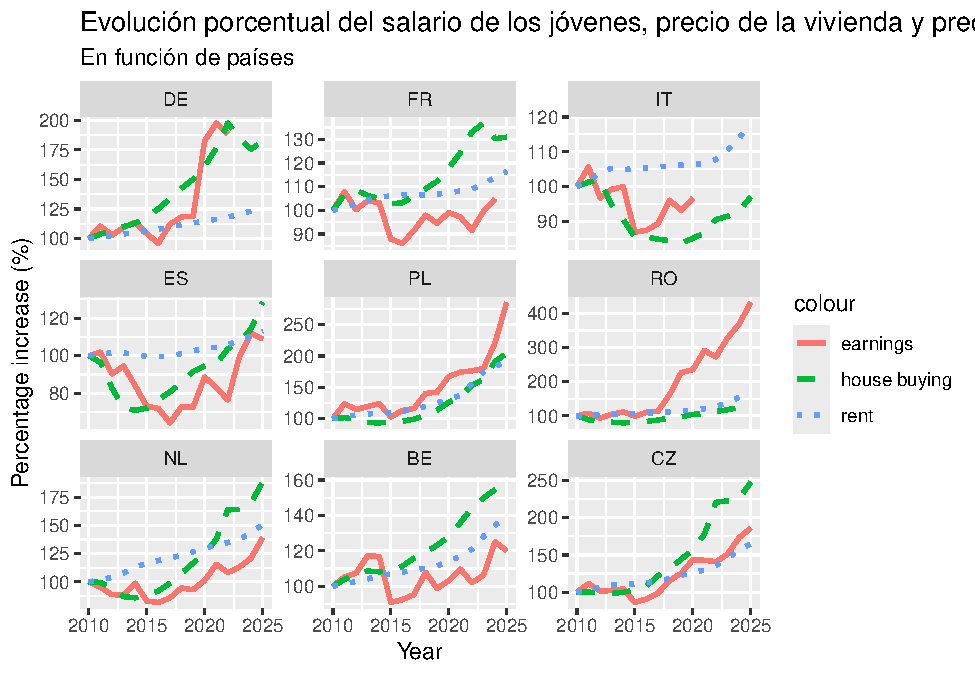
\includegraphics[keepaspectratio]{ProyectoAED_files/figure-latex/unnamed-chunk-29-1.pdf}}

\begin{Shaded}
\begin{Highlighting}[]
\FunctionTok{ggsave}\NormalTok{(}\StringTok{\textquotesingle{}results/viviendas\_salarios.pdf\textquotesingle{}}\NormalTok{, }\AttributeTok{width =} \DecValTok{14}\NormalTok{, }\AttributeTok{height =} \DecValTok{10}\NormalTok{, }\AttributeTok{dpi =} \DecValTok{300}\NormalTok{)}
\end{Highlighting}
\end{Shaded}

\begin{Shaded}
\begin{Highlighting}[]
\FunctionTok{ggplot}\NormalTok{(}\AttributeTok{data =} \FunctionTok{filter}\NormalTok{(jovenes.df, country }\SpecialCharTok{!=} \StringTok{\textquotesingle{}EL\textquotesingle{}}\NormalTok{, year }\SpecialCharTok{\textgreater{}=} \DecValTok{2005} \SpecialCharTok{\&}\NormalTok{ year }\SpecialCharTok{\textless{}=} \DecValTok{2025}\NormalTok{)) }\SpecialCharTok{+} 
  \FunctionTok{geom\_line}\NormalTok{(}\FunctionTok{aes}\NormalTok{(}\AttributeTok{x =}\NormalTok{ year, }\AttributeTok{y =}\NormalTok{ earn.prop.house, }\AttributeTok{color =} \StringTok{\textquotesingle{}by house prices\textquotesingle{}}\NormalTok{), }\AttributeTok{linewidth =} \DecValTok{1}\NormalTok{, }\AttributeTok{na.rm =} \ConstantTok{TRUE}\NormalTok{) }\SpecialCharTok{+} 
  \FunctionTok{geom\_line}\NormalTok{(}\FunctionTok{aes}\NormalTok{(}\AttributeTok{x =}\NormalTok{ year, }\AttributeTok{y =}\NormalTok{ earn.prop.rent, }\AttributeTok{color =} \StringTok{\textquotesingle{}by rent\textquotesingle{}}\NormalTok{), }\AttributeTok{linewidth =} \DecValTok{1}\NormalTok{, }\AttributeTok{na.rm =} \ConstantTok{TRUE}\NormalTok{) }\SpecialCharTok{+} \FunctionTok{facet\_wrap}\NormalTok{(.}\SpecialCharTok{\textasciitilde{}}\NormalTok{country, }\AttributeTok{nrow =} \DecValTok{4}\NormalTok{, }\AttributeTok{scales =} \StringTok{\textquotesingle{}free\_y\textquotesingle{}}\NormalTok{) }\SpecialCharTok{+} \FunctionTok{labs}\NormalTok{(}\AttributeTok{title =} \StringTok{\textquotesingle{}Evolución del salario real en proporción al precio de la vivienda y del alquiler\textquotesingle{}}\NormalTok{, }\AttributeTok{subtitle =} \StringTok{\textquotesingle{}En función de países\textquotesingle{}}\NormalTok{) }\SpecialCharTok{+} \FunctionTok{xlab}\NormalTok{(}\StringTok{\textquotesingle{}Year\textquotesingle{}}\NormalTok{) }\SpecialCharTok{+} \FunctionTok{ylab}\NormalTok{(}\StringTok{\textquotesingle{}Percentage increase (\%)\textquotesingle{}}\NormalTok{)}
\end{Highlighting}
\end{Shaded}

\pandocbounded{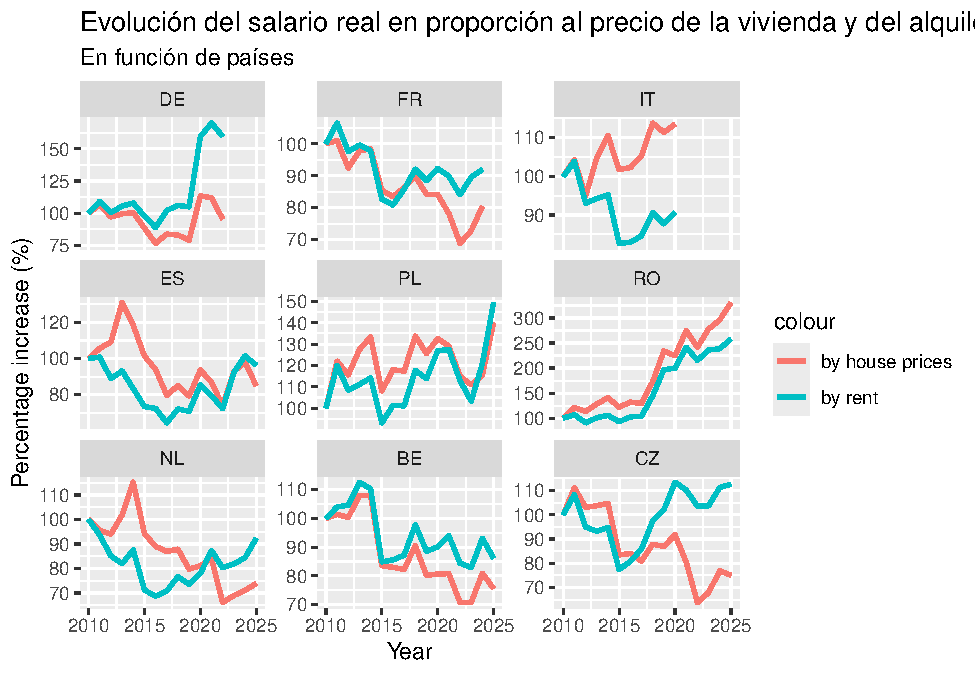
\includegraphics[keepaspectratio]{ProyectoAED_files/figure-latex/unnamed-chunk-30-1.pdf}}

\begin{Shaded}
\begin{Highlighting}[]
\FunctionTok{ggsave}\NormalTok{(}\StringTok{\textquotesingle{}results/proporcion\_salario.pdf\textquotesingle{}}\NormalTok{, }\AttributeTok{width =} \DecValTok{14}\NormalTok{, }\AttributeTok{height =} \DecValTok{10}\NormalTok{, }\AttributeTok{dpi =} \DecValTok{300}\NormalTok{)}
\end{Highlighting}
\end{Shaded}

\begin{Shaded}
\begin{Highlighting}[]
\NormalTok{medias.long }\OtherTok{\textless{}{-}}\NormalTok{ medias.pais }\SpecialCharTok{\%\textgreater{}\%} \FunctionTok{pivot\_longer}\NormalTok{(}\FunctionTok{all\_of}\NormalTok{(vars.pct), }\AttributeTok{names\_to =} \StringTok{\textquotesingle{}variable\textquotesingle{}}\NormalTok{, }\AttributeTok{values\_to =} \StringTok{\textquotesingle{}media\textquotesingle{}}\NormalTok{) }\SpecialCharTok{\%\textgreater{}\%} \FunctionTok{mutate}\NormalTok{(}\AttributeTok{country =} \FunctionTok{factor}\NormalTok{(country, }\AttributeTok{levels =} \FunctionTok{as.character}\NormalTok{(medias.pais}\SpecialCharTok{$}\NormalTok{country[}\FunctionTok{order}\NormalTok{(medias.pais}\SpecialCharTok{$}\NormalTok{house.pct)])), }\AttributeTok{variable =} \FunctionTok{factor}\NormalTok{(variable, }\AttributeTok{levels =}\NormalTok{ vars.pct))}

\FunctionTok{ggplot}\NormalTok{(medias.long, }\FunctionTok{aes}\NormalTok{(}\AttributeTok{x =}\NormalTok{ country, }\AttributeTok{y =}\NormalTok{ media, }\AttributeTok{color =}\NormalTok{ variable, }\AttributeTok{shape =}\NormalTok{ variable)) }\SpecialCharTok{+} \FunctionTok{geom\_point}\NormalTok{(}\AttributeTok{size =} \DecValTok{3}\NormalTok{) }\SpecialCharTok{+} \FunctionTok{geom\_hline}\NormalTok{(}\AttributeTok{yintercept =} \DecValTok{0}\NormalTok{, }\AttributeTok{linetype =} \DecValTok{2}\NormalTok{) }\SpecialCharTok{+} \FunctionTok{labs}\NormalTok{(}\AttributeTok{title =} \StringTok{\textquotesingle{}Media del aumento anual por país\textquotesingle{}}\NormalTok{, }\AttributeTok{subtitle =} \FunctionTok{paste0}\NormalTok{(}\StringTok{\textquotesingle{}Ventana común \textquotesingle{}}\NormalTok{, year.ini, }\StringTok{\textquotesingle{}{-}\textquotesingle{}}\NormalTok{, year.fin, }\StringTok{\textquotesingle{}; países ordenados por el aumento de la vivienda\textquotesingle{}}\NormalTok{)) }\SpecialCharTok{+} \FunctionTok{xlab}\NormalTok{(}\StringTok{\textquotesingle{}Country\textquotesingle{}}\NormalTok{) }\SpecialCharTok{+} \FunctionTok{ylab}\NormalTok{(}\StringTok{\textquotesingle{}Mean annual increase (\%)\textquotesingle{}}\NormalTok{)}
\end{Highlighting}
\end{Shaded}

\pandocbounded{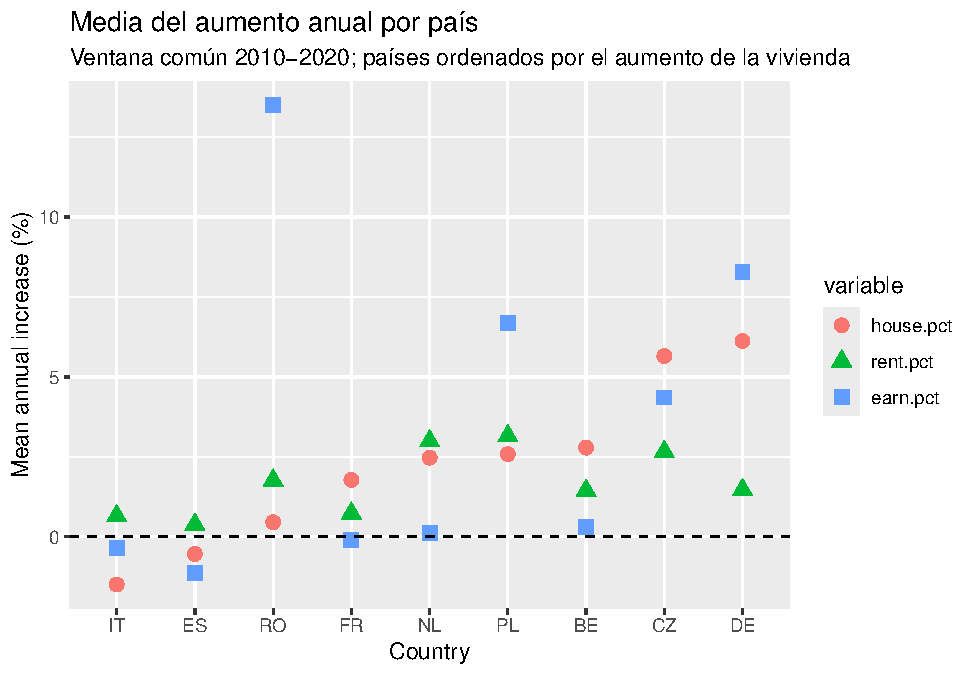
\includegraphics[keepaspectratio]{ProyectoAED_files/figure-latex/unnamed-chunk-31-1.pdf}}

\begin{Shaded}
\begin{Highlighting}[]
\FunctionTok{ggsave}\NormalTok{(}\StringTok{\textquotesingle{}results/univ\_aumentos\_medias.pdf\textquotesingle{}}\NormalTok{, }\AttributeTok{width =} \DecValTok{14}\NormalTok{, }\AttributeTok{height =} \DecValTok{10}\NormalTok{, }\AttributeTok{dpi =} \DecValTok{300}\NormalTok{)}
\end{Highlighting}
\end{Shaded}


\bibliography{mybibfile.bib}



\end{document}
